%
% OpenDCS Proposal
%
% Author: Geoff Johnson
%
% To compile: pdflatex --shell-escape --synctex=1 --interaction=nonstopmode report.tex
%

\documentclass[11pt]{article}

\usepackage[titles]{tocloft}
\usepackage{verbatim}
\usepackage[pdftex]{graphics,graphicx}
\usepackage{wrapfig}
\usepackage[export]{adjustbox}
\usepackage{booktabs}
\usepackage{pdfpages}
\usepackage{float}
\usepackage{amssymb}
\usepackage{mathtools}
\usepackage{svg}
\usepackage{tikz}
\usepackage{listings,lstautogobble}
\usepackage[tablegrid]{vhistory}
\usetikzlibrary{arrows}

\usepackage[backend=biber]{biblatex}
%\bibliography{references}
\addbibresource{references.bib}

\usepackage{hyperref}
\hypersetup{%
  pdfauthor={Geoff Johnson},
  pdftitle={OpenDCS Project Report},
  pdfsubject={Project Report},
  pdfkeywords={OpenDCS Project Report},
  colorlinks=true,
  linkcolor=black,
  urlcolor=blue
}

% Change listing setup.
\definecolor{sol-basic}{RGB}{101,123,131} % Base0
\definecolor{sol-comment}{RGB}{147,161,161} % Base1
\definecolor{sol-keyword}{RGB}{133,153,0} % Green
\definecolor{sol-string}{RGB}{203,75,22} % Orange
\definecolor{sol-emph}{RGB}{211,54,130} % Magenta
\definecolor{sol-background}{RGB}{253,246,227} % Base3

\lstset{%
  language=xml,
  backgroundcolor=\color{sol-background},
  identifierstyle=\ttfamily,
  basicstyle=\footnotesize\ttfamily\color{sol-basic},
  keywordstyle=\color{sol-keyword},
  commentstyle=\color{sol-comment},
  stringstyle=\color{sol-string},
  emph={dcs,objects,object,property},
  emphstyle={\color{sol-emph}},
  tabsize=4,
  aboveskip={1.5\baselineskip},
  columns=fixed,
  inputencoding=utf8,
  extendedchars=true,
  breaklines=true,
  prebreak = \raisebox{0ex}[0ex][0ex]{\ensuremath{\hookleftarrow}},
  frame=single,
  showtabs=false,
  showspaces=false,
  showstringspaces=false,
  numbers=left,
  numberstyle=\tiny,
  breakatwhitespace=true,
  title=\lstname,
  literate={│}{{\textSFxi}}1 {└}{{\textSFii}}1 {├}{{\textSFviii}}1 {─}{{\textSFx}}1,
  autogobble=true,
}

\lstdefinelanguage{JavaScript}{%
  keywords={typeof, new, true, false, catch, function, return, null, catch, switch, var, if, in, while, do, else, case, break},
  keywordstyle=\color{sol-keyword}\bfseries,
  ndkeywords={class, export, boolean, throw, implements, import, this},
  ndkeywordstyle=\color{sol-keyword}\bfseries,
  identifierstyle=\color{sol-basic},
  sensitive=false,
  comment=[l]{//},
  morecomment=[s]{/*}{*/},
  commentstyle=\color{sol-comment}\ttfamily,
  stringstyle=\color{sol-string}\ttfamily,
  morestring=[b]',
  morestring=[b]"
}

% Packages used for appendices.
\usepackage{appendix}
\usepackage{listings}
\usepackage{color}
\definecolor{light-gray}{gray}{0.95}
\definecolor{listinggray}{gray}{0.9}
\definecolor{lbcolor}{rgb}{0.9,0.9,0.9}
\definecolor{light-blue}{rgb}{0.6,0.720,0.85}

% The default margins are too wide all the way around, reset them.
\setlength{\topmargin}{-.5in}
\setlength{\textheight}{9in}
\setlength{\oddsidemargin}{0in}
\setlength{\textwidth}{6.5in}

% Change paragraph formatting.
\setlength{\parindent}{0pt}
\setlength{\parskip}{2ex}

% Add paragraph as a section number
\setcounter{secnumdepth}{4}

% Fix list indentation for requirements
%\usepackage{enumitem}
%\setlist[requirement]{leftmargin=\parindent,labelindent=\parindent} % doesn't work

\begin{document}
\nocite{*}

  \title{%
    OpenDCS $-$ An Open Distributed Control System\vspace{2em}
  }

  \author{%
    Geoff Johnson \vspace{0.5em} \\
    geoff.jay@gmail.com \vspace{0.5em} \\
    A00533481 \vspace{0.5em} \\
    COMP8045 \vspace{0.5em}
  }

  \maketitle
  \thispagestyle{empty}
  \newpage
  \mbox{}
  \thispagestyle{empty}

  \newpage
  \addtocounter{page}{-1}
  \pagenumbering{roman}
  \tableofcontents

  \newpage
  \pagenumbering{arabic}

  % XXX fill in or omit sections as needed, for now just blasting ideas

  \section{Project Description}\label{sec:desc}

  \subsection{Background}\label{sec:desc-bg}

    \subsubsection{Student}\label{sec:desc-bg-student}

      Geoff Johnson is a student of the BCIT Computer Systems Bachelor's degree.
      Prior to this he obtained a diploma of Computer Systems Technology from
      Camosun college in Victoria in 2001, as well as a diploma in Robotics and
      Automation Technology from BCIT in 2006.

      For the past 10 years Geoff has worked in Burnaby for the fluid mechanics
      research and development company Coanda where he is responsible for managing
      the IT operations, as well as managing and contributing to control system
      software development. This software is used to interface with industrial
      instrumentation, perform automated feedback control of plant processes,
      and capture data to log files at upwards of 100,000 samples per second.

    \subsubsection{Company}\label{sec:desc-bg-company}

      Coanda is an engineering research and development company specializing in
      industrial fluid dynamics and related technologies. They have been in
      business for close to 20 years providing services in process flow modelling,
      design optimization, and custom instrumentation to name a few. For more
      information their website is \url{https://www.coanda.ca}.

    \subsubsection{History}\label{sec:desc-bg-project}

      The project that was proposed, and is the subject of this report, was the
      reproduction of an existing piece of software used to measure and control
      physical processes. The software that this project seeks to improve upon
      is comprised of two software projects, a library of objects that abstract
      components of a data acquisition and control system, and a GUI application
      that functions as an operator panel.

      The first is a library of objects that abstracts the data acquisition
      hardware as various types of measurement channels, it handles logging
      to both CSV files as well as databases, feedback control loop
      calculations using the PID (Proportional Integral Derivative) equation,
      and handles the creation of object hierarchy through a class builder
      using XML as the input. This library, libcld, is an open source project
      hosted in a git repository at \url{https://github.com/geoffjay/libcld}.

      The second piece of software is a user facing GUI application developed for
      the GNOME system. It interfaces with libcld, hereafter referred to as
      CLD (Control, Logging, and Data Acquisition), using a single context to
      provide the data necessary to update the interface view. This application
      has also been released as open source and is hosted in a git repository
      at \url{https://github.com/coanda/dactl}.

  \subsection{Proposed Solution}\label{sec:desc-soln}

    Performing all of the work in a single application for data acquisition,
    feedback control, and data logging is open to a variety of issues. Doing so
    limits hardware scalability, places critical operations onto systems running
    desktop software, and ties high reliability functions like plant control in
    the same process as the front end that the end user operates. These are just
    a few of the more obvious problems.

    The system being proposed in this document is one that implements all of
    the hardware access and logging functionality as micro-services that run as
    processes detached from the plant operators that interact with the GUI
    application. This server software will use an existing library to interface
    with the data acquisition hardware as well as perform the control and
    logging tasks, this aspect of the software is a reimplementation of work
    that already exists in an application that is currently in use.

    New functionality that is planned is the definition and minimal
    implementation of a REST API, a messaging system for streaming data, and a
    configuration definition to allow for the reconfiguration of the daemon. The
    REST API is meant to provide a means for clients to make simple requests of
    the system like read a single measurement value or change a property value
    of one of the internal objects. ZeroMQ is to be used to implement the
    messaging system, it has several high level features including publish and
    subscribe socket types that can be used for a streaming data system, a
    request/reply structure for a higher performance version of the REST API,
    and a structure for bridging communications to allow for the reconfiguration
    of the server as a proxy or slave node in a distributed system.


  \newpage
  \section{Technology}\label{sec:tech}

  Various technologies will be used to develop OpenDCS, this section is intended
  to provide some common terms and expressions used throughout the document.

  \subsection{ZeroMQ}\label{sec:tech-zmq}

    ZeroMQ is a library that provides a means of creating systems that have
    distributed messaging. From the website (\url{http://zeromq.com}) it offers
    the ability to:

    \begin{itemize}
      \item Connect your code in any language, on any platform.
      \item Carries messages across inproc, IPC, TCP, TIPC, multicast.
      \item Smart patterns like pub-sub, push-pull, and router-dealer.
      \item High-speed asynchronous I/O engines, in a tiny library.
      \item Backed by a large and active open source community.
      \item Supports every modern language and platform.
      \item Build any architecture: centralized, distributed, small, or large.
    \end{itemize}

    Socket types are available to make several patterns possible such as
    Request-Reply (REQ-REP), Publish-Subscribe (PUB-SUB), Parallel Pipelines,
    and Fair Queuing among others. OpenDCS services will initially only be
    developed to use the PUB-SUB and the REQ-REP patterns, but could eventually
    use others. The ability to extend to these others in the future was the
    reason for selecting this library over something else, such as TCP or UDP
    sockets on their own.

    \paragraph{PUB-SUB Pattern}

      With this form of messaging the publisher sends the message, and the
      subscriber receives them. Messages are meant to be characterized such
      that they be sent without any knowledge of which subscribers will receive
      them, if any at all. Messages can be filtered by the subscriber which
      allows them to receive only the subset that is desired.

      \begin{figure}[H]
        \begin{center}
          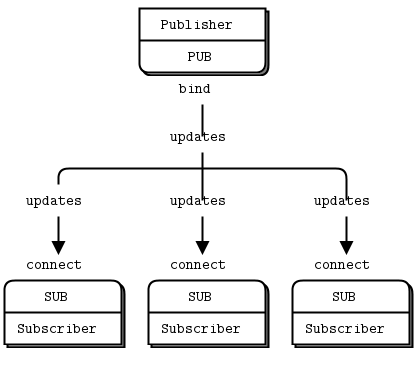
\includegraphics[width=0.5\textwidth]{figures/pub-sub-pattern}
        \end{center}
      \end{figure}

    \paragraph{REQ-REP Pattern}

      This pattern is one of the basic methods that is used in network
      application development to communicate between systems. With this type a
      connection is made and there are a series of transactions until the
      request is complete and a response is provided. A simple example of this
      is browsing a web page, a person using a web browser requests a page and
      the server responds with the page content for the browser to render

      \begin{figure}[H]
        \begin{center}
          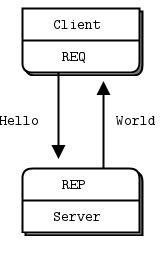
\includegraphics[width=0.25\textwidth]{figures/req-rep-pattern}
        \end{center}
      \end{figure}

  \subsection{Vala}\label{sec:tech-vala}

    Vala is a programming language that aims to bring modern programming
    language features without imposing any runtime requirements and without
    using a different ABI compared to applications and libraries written in
    C~\cite{Vala2016}.


  \newpage
  \section{Requirements}\label{sec:req}

  The stakeholders that have been identified from Coanda are:

  \begin{table}[H]
    \centering
    \begin{tabular}{l p{6cm} p{6cm}}
      \toprule
      Name & Organization Role & Project Role \\ [0.5ex]
      \midrule
      Geoff Johnson & Software Developer        & Project Lead \\
      Stephen Roy   & Software Developer        & Contributor \\
      Scott Webster & Research Scientist        & Requirements Contributor \\
      Thomas Depew  & Instrumentation Scientist & Requirements Contributor \\
      Bernie LeSage & Chief Operations Officer  & Project Reviewer \\
      \bottomrule
    \end{tabular}
    \caption{Project Stakeholders}\label{tab:stakeholders}
  \end{table}

  \subsection{Raw List from Project Stakeholders}\label{sec:req-sh}

    During a meeting with project contributors at the beginning of the
    requirements gathering process the question ``What would you like to be
    able to do with the system'' was posed. A summary of the responses is
    given below in Table~\ref{tab:requirements} where each may or may not
    be directly applicable to this stage of the project. For instance elements
    of the user interface that are of interest are not a component of this
    work, instead what will be attempted with these is an analysis of how the
    system can be structured to support that development in the future.

    \begin{table}[H]
      \centering
      \begin{tabular}{l p{11cm} p{3cm}}
        \toprule
        Number & Description & Priority (1-5)\newline 1 is highest \\ [0.5ex]
        \midrule
         1 & Devices must be loaded as plugins & 1 \\
         2 & Want to run any service on a RaspberryPI & 3 \\
         3 & Like to run HMI on Windows systems & 5 \\
         4 & Messages from services should be test-able using curl & 2 \\
         5 & Data stream monitoring should be possible using tcpdump-like utility & 2 \\
         6 & Message compression and decompression using msgpack is desired & 3 \\
         7 & Configuration for all components needs to be consistent and similar to existing format used by libcld and dactl & 1 \\
         8 & About/help systems for components should show versions and patches in use & 2 \\
         9 & Must be able to develop plugins in Python as well as C/Vala & 1 \\
        10 & Plugin skeletons should be possible to generate from templates & 3 \\
        11 & Must be able to run any individual component on the same or separate host & 2 \\
        12 & Plotting data in some format is a must & 2 \\
        13 & The data logger data must be query-able from that service over a given date and time range & 1 \\
        \bottomrule
      \end{tabular}
      \caption{Initial Requirements List}\label{tab:requirements}
    \end{table}

    \begin{table}[H]
      \centering
      \begin{tabular}{l p{11cm} p{3cm}}
        \toprule
        Number & Description & Priority (1-5)\newline 1 is highest \\ [0.5ex]
        \midrule
        14 & Time synchronization between the services that run on different computers should be possible & 5 \\
        15 & Some method of broadcasting to the services should be provided for messages that apply to the system as a whole & 3 \\
        16 & Must be able to acquire data from different devices and device types & 1 \\
        17 & Logging data to plain text is a must, to special binary formats is a nice to have & 1 \\
        18 & Must be able to perform feedback control of actuators using acquired data & 1 \\
        19 & Documentation needs to be available to provide end users the know how to launch the services & 3 \\
        20 & Documentation needs to be available to describe how to configure the services & 3 \\
        21 & The build process should allow you to compile and install individual components as well as the system as a whole & 4 \\
        22 & Data needs to be available over networked computers & 2 \\
        23 & A well structured messaging format needs to be defined for other services and consumers to adhere to & 2 \\
        24 & ZeroMQ should be used as the message queue system & 1 \\
        25 & Services should also provide a RESTful API to make their information available to other software regardless of the language used to develop it & 2 \\
        26 & Data acquisition devices need to be developed as plugins that are loaded into the DAQ service & 1 \\
        27 & Data logging backends like XML or databases need to be developed as plugins that are loaded into the data logging service & 1 \\
        28 & Feedback controllers need to be developed as plugins that are loaded into the control service & 1 \\
        29 & Would be nice to be able to test and possibly distribute the different services as Dockerized applications & 4 \\
        30 & Should be able to build and load the various plugins for the system using documentation provided & 3 \\
        31 & Should be able to install any system component by following the documentation provided & 1 \\
        32 & Should be able to configure any system component by following the documentation provided & 2 \\
        33 & Should be able to test any system component by following the documentation provided & 3 \\
        \bottomrule
      \end{tabular}
      \caption{Initial Requirements List Continued}\label{tab:requirements}
    \end{table}

  \subsection{Analysis}\label{sec:req-analyze}

  \subsection{System Requirements Specifications}\label{sec:req-srs}

    The system requirements for OpenDCS are described in this section, it
    contains information about the functionality of the system as a whole.
    OpenDCS is a platform that has the potential to integrate with electrical
    and mechanical systems so it is necessary to comment on the software
    interactions with such systems, but due to the nature of the design it
    would be impossible to enforce strict rules governing external systems
    that are mechanical, electrical and software.

    This section contains all of the functional and quality requirements of
    the system. A detailed description of the system and all its features is
    given. The following is a list of the abbreviations and acronyms used to
    document these requirements.

    \begin{itemize}
      \setlength{\itemindent}{.5in}
      \itemsep .15em
      \item[ID:] requirement identifier
      \item[TAG:] short form of name
      \item[DESC:] description
      \item[RAT:] rationale
      \item[DEP:] dependencies
      \item[GIST:] rough summary
      \item[SCALE:] the unit for the req to be measured in
      \item[METER:] the way in which the measurement will be performed, can specify test
      \item[PAST:] benchmark typ. for products dev'd in past
      \item[REC:] (record) benchmark represents best value achieved for meter
      \item[MUST:] minimal goal value
      \item[PLAN:] desired goal value
      \item[WISH:] ideal goal value
    \end{itemize}

    \subsubsection{External Interface Requirements}\label{sec:req-srs-func}

      \paragraph{User Interfaces}

      \paragraph{Hardware Interfaces}

        \begin{itemize}
          \setlength{\itemindent}{.5in}
          \itemsep .15em
          \item[ID:] HWIR-0001
          \item[TAG:] RS-232 Serial Port
          \item[DESC:] A serial port data acquisition device should be able
            to connect to the system.
          \item[RAT:] Plugin device development will make use of serial port
            core functionality.
        \end{itemize}

        \begin{itemize}
          \setlength{\itemindent}{.5in}
          \itemsep .15em
          \item[ID:] HWIR-0002
          \item[TAG:] Ethernet
          \item[DESC:] The system shall communicate using 10BASE-T,
            100BASE-TX and 1000BASE-T.
          \item[RAT:] The physical system components connect to the network
            using Ethernet.
        \end{itemize}

        \begin{itemize}
          \setlength{\itemindent}{.5in}
          \itemsep .15em
          \item[ID:] HWIR-0003
          \item[TAG:] Number of Ethernet Ports
          \item[DESC:] The number of ports required shall depend on how the
            system configuration for a particular application and whether it
            needs to connect to remote hardware.
          \item[RAT:] Multiple physical hosts can be used to configure a
            system of services.
        \end{itemize}

        \begin{itemize}
          \setlength{\itemindent}{.5in}
          \itemsep .15em
          \item[ID:] HWIR-0004
          \item[TAG:] Processor speed
          \item[DESC:] The system components shall each have a 400 MHz or
            faster processor.
          \item[RAT:] The software requires a reasonably fast processor to
            handle the data and run a user interface.
        \end{itemize}

        \begin{itemize}
          \setlength{\itemindent}{.5in}
          \itemsep .15em
          \item[ID:] HWIR-0005
          \item[TAG:] Display
          \item[DESC:] A 1920 x 1080 (16:9) monitor should be used.
          \item[RAT:] A good user experience that represents a reasonable
            amount of data necessarily requires a display with sufficient
            resolution.
        \end{itemize}

      \paragraph{Software Interfaces}

        \begin{itemize}
          \setlength{\itemindent}{.5in}
          \itemsep .15em
          \item[ID:] SWIR-0001
          \item[TAG:] Operating System
          \item[DESC:] The software architecture shall be 64-bit GNU/Linux
            (e.g. Fedora 25)
          \item[RAT:] The system is intended to be compiled with modern
            software dependencies available in newer Linux distributions.
        \end{itemize}

      \paragraph{Communications Interfaces}

        \begin{itemize}
          \setlength{\itemindent}{.5in}
          \itemsep .15em
          \item[ID:] CIR-0001
          \item[TAG:] ZeroMQ
          \item[DESC:] The system shall use ZeroMQ for publishing and
            subscribing to service data, and to request and reply to
            individual components.
          \item[RAT:] A messaging system is required for easily extending the
            service oriented architecture, ZeroMQ offers a lot of options for
            future concepts.
        \end{itemize}

        \begin{itemize}
          \setlength{\itemindent}{.5in}
          \itemsep .15em
          \item[ID:] CIR-0002
          \item[TAG:] REST
          \item[DESC:] Each service of the system shall provide a RESTful API
            for data access to external components that need/prefer to use
            HTTP requests.
          \item[RAT:] Having this API available to application developers
            simplifies the time required to do simple tasks.
        \end{itemize}

    \subsubsection{Functional Requirements}\label{sec:req-srs-func}

      \paragraph{Common Requirements}

        \begin{itemize}
          \setlength{\itemindent}{.5in}
          \itemsep .15em
          \item[ID:] FR-0001
          \item[TAG:] Connectivity
          \item[DESC:] Requirements that enable communication between and are
            common to all system components that shall be met.
          \item[RAT:] Interoperability of the system components requires a
            common messaging queue.
          \item[DEP:] FR-0002, FR-0003, FR-0004
        \end{itemize}

        \begin{itemize}
          \setlength{\itemindent}{.5in}
          \itemsep .15em
          \item[ID:] FR-0002
          \item[TAG:] Publishing Socket
          \item[DESC:] A configurable ZeroMQ publishing socket shall be
            available.
          \item[RAT:] A service shall be able to publish data on a ZeroMQ
            socket.
          \item[DEP:] none
        \end{itemize}

        \begin{itemize}
          \setlength{\itemindent}{.5in}
          \itemsep .15em
          \item[ID:] FR-0003
          \item[TAG:] Subscribing Socket
          \item[DESC:] A configurable ZeroMQ subscribing socket shall be
            available.
          \item[RAT:] A service can subscribe to published data from other
            system components.
          \item[DEP:] none
        \end{itemize}

        \begin{itemize}
          \setlength{\itemindent}{.5in}
          \itemsep .15em
          \item[ID:] FR-0004
          \item[TAG:] Request/Reply Socket
          \item[DESC:] A ZeroMQ request/reply socket shall be available.
          \item[RAT:] A service can request and receive data from a connected
            system component.
          \item[DEP:] none
        \end{itemize}

        \begin{itemize}
          \setlength{\itemindent}{.5in}
          \itemsep .15em
          \item[ID:] FR-0005
          \item[TAG:] Device Plugin System
          \item[DESC:] A libpeas plugin system must be available to load data
            acquisition devices.
          \item[RAT:] The data acquisition service will get its data to
            transmit from device plugins that are loaded at runtime.
          \item[DEP:] none
        \end{itemize}

        \begin{itemize}
          \setlength{\itemindent}{.5in}
          \itemsep .15em
          \item[ID:] FR-0006
          \item[TAG:] Logging Backend Plugin System
          \item[DESC:] A libpeas plugin system must be available to load data
            logging backends.
          \item[RAT:] The data logging service will log the data it receives
            to backend plugins that are loaded at runtime.
          \item[DEP:] none
        \end{itemize}

        \begin{itemize}
          \setlength{\itemindent}{.5in}
          \itemsep .15em
          \item[ID:] FR-0007
          \item[TAG:] Feedback Controller Plugin System
          \item[DESC:] A libpeas plugin system must be available to load
            feedback controllers.
          \item[RAT:] The feedback control service will use data that it
            receives to perform feedback control using plugins that are
            loaded at runtime.
          \item[DEP:] none
        \end{itemize}

      \paragraph{Data Acquisition}

        \begin{itemize}
          \setlength{\itemindent}{.5in}
          \itemsep .15em
          \item[ID:] DSFR-0001
          \item[TAG:] Data acquisition common system requirements
          \item[DESC:] The common service requirements shall be met.
          \item[RAT:]
          \item[DEP:] FR-0001
        \end{itemize}

        \begin{itemize}
          \setlength{\itemindent}{.5in}
          \itemsep .15em
          \item[ID:] DSFR-0002
          \item[TAG:] Publish Data Messages
          \item[DESC:] Data messages shall be published on the socket
            containing channel measurements, timestamps, and broadcast
            status/warnings.
          \item[RAT:]
          \item[DEP:] FR-0002
        \end{itemize}

        \begin{itemize}
          \setlength{\itemindent}{.5in}
          \itemsep .15em
          \item[ID:] DSFR-0003
          \item[TAG:] Subscribe to Data Messages
          \item[DESC:] The data acquisition system component shall be able to
            subscribe to published messages.
          \item[RAT:]
          \item[DEP:] FR-0003
        \end{itemize}

        \begin{itemize}
          \setlength{\itemindent}{.5in}
          \itemsep .15em
          \item[ID:] DSFR-0004
          \item[TAG:] Start
          \item[DESC:] The data acquisition system component shall start
            publishing data in response to a request to do so if it has not
            already started.
          \item[RAT:]
          \item[DEP:] FR-0002
        \end{itemize}

        \begin{itemize}
          \setlength{\itemindent}{.5in}
          \itemsep .15em
          \item[ID:] DSFR-0005
          \item[TAG:] Stop
          \item[DESC:] The data acquisition system component shall stop
            publishing data in response to a request to do so.
          \item[RAT:]
          \item[DEP:] FR-0002
        \end{itemize}

        \begin{itemize}
          \setlength{\itemindent}{.5in}
          \itemsep .15em
          \item[ID:] DSFR-0006
          \item[TAG:] Automatic Start
          \item[DESC:] The data acquisition system component shall start
            publishing data immediately.
          \item[RAT:]
          \item[DEP:] FR-0002
        \end{itemize}

      \paragraph{Data Logging}

        \begin{itemize}
          \setlength{\itemindent}{.5in}
          \itemsep .15em
          \item[ID:] LSFR-0001
          \item[TAG:] Data logging common system requirements
          \item[DESC:] The common service requirements shall be met.
          \item[RAT:]
          \item[DEP:] FR-0001
        \end{itemize}

        \begin{itemize}
          \setlength{\itemindent}{.5in}
          \itemsep .15em
          \item[ID:] LSFR-0002
          \item[TAG:] Publish backend malfunction warning
          \item[DESC:] Data messages shall be published as a warning when its
            back end data storage is not functioning.
          \item[RAT:] To allow the subscribing GUI interface to alert the
            user.
          \item[DEP:] FR-0002
        \end{itemize}

        \begin{itemize}
          \setlength{\itemindent}{.5in}
          \itemsep .15em
          \item[ID:] LSFR-0003
          \item[TAG:] Subscribe to published data from data acquisition system.
          \item[DESC:]
          \item[RAT:]
          \item[DEP:] FR-0003
        \end{itemize}

      \paragraph{Feedback Control}

        \begin{itemize}
          \setlength{\itemindent}{.5in}
          \itemsep .15em
          \item[ID:] CSFR-0001
          \item[TAG:] Feedback control common system requirements
          \item[DESC:] The common service requirements shall be met.
          \item[RAT:]
          \item[DEP:] FR-0001
        \end{itemize}

        \begin{itemize}
          \setlength{\itemindent}{.5in}
          \itemsep .15em
          \item[ID:] CSFR-0002
          \item[TAG:] Subscribe to input data
          \item[DESC:] The feedback control system will subscribe to
            published data from the data acquisition system and filter out
            the channel measurement data that it needs.
          \item[RAT:] Input data is required for its calculations.
          \item[DEP:] FR-0003
        \end{itemize}

        \begin{itemize}
          \setlength{\itemindent}{.5in}
          \itemsep .15em
          \item[ID:] CSFR-0003
          \item[TAG:] Publish output data
          \item[DESC:] The feedback control system shall publish the data
            resultant of it calculations.
          \item[RAT:] Output data is required to control process variable
            outputs.
          \item[DEP:] FR-0002
        \end{itemize}

        \begin{itemize}
          \setlength{\itemindent}{.5in}
          \itemsep .15em
          \item[ID:] CSFR-0004
          \item[TAG:] Perform Feedback Control
          \item[DESC:] Feedback control of hardware performed by the service
            must be possible.
          \item[RAT:] Hardware control is fundamental to a distributed
            control system.
          \item[DEP:] FR-0002, FR-0003, CSFR-0002, CSFR-0003
        \end{itemize}

    \subsubsection{Non-Functional Requirements}\label{sec:req-srs-func}

      \paragraph{Performance}

        The requirements in this section provide a detailed specification of
        the user interaction with the software and measurements placed on the
        system performance.

        Usage of the data log query feature

        \begin{itemize}
          \setlength{\itemindent}{.5in}
          \itemsep .15em
          \item[ID:] QR-0001
          \item[GIST:] Data log query response time.
          \item[SCALE:]
          \item[METER:]
          \item[MUST:]
          \item[PLAN:]
          \item[WISH:]
        \end{itemize}

        Usage of the data acquisition message publish feature

        \begin{itemize}
          \setlength{\itemindent}{.5in}
          \itemsep .15em
          \item[ID:] QR-0002
          \item[GIST:]
          \item[SCALE:]
          \item[METER:]
          \item[MUST:]
          \item[PLAN:]
          \item[WISH:]
        \end{itemize}

        Usage of the data acquisition message subscribe feature

        \begin{itemize}
          \setlength{\itemindent}{.5in}
          \itemsep .15em
          \item[ID:] QR-0003
          \item[GIST:]
          \item[SCALE:]
          \item[METER:]
          \item[MUST:]
          \item[PLAN:]
          \item[WISH:]
        \end{itemize}

        Configuration modification request response time

        \begin{itemize}
          \setlength{\itemindent}{.5in}
          \itemsep .15em
          \item[ID:] QR-0004
          \item[GIST:]
          \item[SCALE:]
          \item[METER:]
          \item[MUST:]
          \item[PLAN:]
          \item[WISH:]
        \end{itemize}

        Configuration information request response time

        \begin{itemize}
          \setlength{\itemindent}{.5in}
          \itemsep .15em
          \item[ID:] QR-0005
          \item[GIST:]
          \item[SCALE:]
          \item[METER:]
          \item[MUST:]
          \item[PLAN:]
          \item[WISH:]
        \end{itemize}

        Sample rate capacity of data acquisition service

        \begin{itemize}
          \setlength{\itemindent}{.5in}
          \itemsep .15em
          \item[ID:] QR-0006
          \item[GIST:]
          \item[SCALE:]
          \item[METER:]
          \item[MUST:]
          \item[PLAN:]
          \item[WISH:]
        \end{itemize}

        Sample rate capacity of data logging service

        \begin{itemize}
          \setlength{\itemindent}{.5in}
          \itemsep .15em
          \item[ID:] QR-0007
          \item[GIST:]
          \item[SCALE:]
          \item[METER:]
          \item[MUST:]
          \item[PLAN:]
          \item[WISH:]
        \end{itemize}

        Sample rate capacity of feedback control service

        \begin{itemize}
          \setlength{\itemindent}{.5in}
          \itemsep .15em
          \item[ID:] QR-0008
          \item[GIST:]
          \item[SCALE:]
          \item[METER:]
          \item[MUST:]
          \item[PLAN:]
          \item[WISH:]
        \end{itemize}

        System dependability of the data acquisition service

        \begin{itemize}
          \setlength{\itemindent}{.5in}
          \itemsep .15em
          \item[ID:] QR-0009
          \item[GIST:] The fault tolerance of the system.
          \item[SCALE:] If the system loses its connection to the building
            network, another connected component, or a malformed message, the
            user should be informed.
          \item[METER:] Measurements obtained from 100 hours of usage during
            testing.
          \item[MUST:] 99\% of the time
          \item[PLAN:] 100\% of the time
          \item[WISH:] 100\% of the time
        \end{itemize}

        System dependability of the data logging service

        \begin{itemize}
          \setlength{\itemindent}{.5in}
          \itemsep .15em
          \item[ID:] QR-0010
          \item[GIST:] The fault tolerance of the system.
          \item[SCALE:] If the system loses its connection to the building
            network, another connected component, or a malformed message, the
            user should be informed.
          \item[METER:] Measurements obtained from 100 hours of usage during
            testing.
          \item[MUST:] 99\% of the time
          \item[PLAN:] 100\% of the time
          \item[WISH:] 100\% of the time
        \end{itemize}

        System dependability of the feedback control service

        \begin{itemize}
          \setlength{\itemindent}{.5in}
          \itemsep .15em
          \item[ID:] QR-0011
          \item[GIST:] The fault tolerance of the system.
          \item[SCALE:] If the system loses its connection to the building
            network, another connected component, or a malformed message, the
            user should be informed.
          \item[METER:] Measurements obtained from 100 hours of usage during
            testing.
          \item[MUST:] 99\% of the time
          \item[PLAN:] 100\% of the time
          \item[WISH:] 100\% of the time
        \end{itemize}

      \paragraph{Design Constraints}

        This section includes the design constraints on the software caused by
        the hardware.

        Network bandwidth

        \begin{itemize}
          \setlength{\itemindent}{.5in}
          \itemsep .15em
          \item[ID:] QR-00
          \item[GIST:]
          \item[SCALE:]
          \item[METER:]
          \item[MUST:]
          \item[PLAN:]
          \item[WISH:]
        \end{itemize}

        Network latency

        \begin{itemize}
          \setlength{\itemindent}{.5in}
          \itemsep .15em
          \item[ID:] QR-00
          \item[GIST:]
          \item[SCALE:]
          \item[METER:]
          \item[MUST:]
          \item[PLAN:]
          \item[WISH:]
        \end{itemize}

        Data acquisition device speed

        \begin{itemize}
          \setlength{\itemindent}{.5in}
          \itemsep .15em
          \item[ID:] QR-00
          \item[GIST:]
          \item[SCALE:]
          \item[METER:]
          \item[MUST:]
          \item[PLAN:]
          \item[WISH:]
        \end{itemize}

        Hard drive read/write speed

        \begin{itemize}
          \setlength{\itemindent}{.5in}
          \itemsep .15em
          \item[ID:] QR-00
          \item[GIST:]
          \item[SCALE:]
          \item[METER:]
          \item[MUST:]
          \item[PLAN:]
          \item[WISH:]
        \end{itemize}

        Application memory usage

        \begin{itemize}
          \setlength{\itemindent}{.5in}
          \itemsep .15em
          \item[ID:] QR-00
          \item[GIST:]
          \item[SCALE:]
          \item[METER:]
          \item[MUST:]
          \item[PLAN:]
          \item[WISH:]
        \end{itemize}

        Application processor usage

        \begin{itemize}
          \setlength{\itemindent}{.5in}
          \itemsep .15em
          \item[ID:] QR-00
          \item[GIST:]
          \item[SCALE:]
          \item[METER:]
          \item[MUST:]
          \item[PLAN:]
          \item[WISH:]
        \end{itemize}

      \paragraph{Software System Attributes}

        Reliability

        \begin{itemize}
          \setlength{\itemindent}{.5in}
          \itemsep .15em
          \item[ID:] QR-00
          \item[GIST:]
          \item[SCALE:]
          \item[METER:]
          \item[MUST:]
          \item[PLAN:]
          \item[WISH:]
        \end{itemize}

        Availability

        \begin{itemize}
          \setlength{\itemindent}{.5in}
          \itemsep .15em
          \item[ID:] QR-00
          \item[GIST:]
          \item[SCALE:]
          \item[METER:]
          \item[MUST:]
          \item[PLAN:]
          \item[WISH:]
        \end{itemize}

        \begin{itemize}
          \setlength{\itemindent}{.5in}
          \itemsep .15em
          \item[ID:] QR-00
          \item[GIST:]
          \item[SCALE:]
          \item[METER:]
          \item[MUST:]
          \item[PLAN:]
          \item[WISH:]
        \end{itemize}

        \begin{itemize}
          \setlength{\itemindent}{.5in}
          \itemsep .15em
          \item[ID:] QR-00
          \item[GIST:]
          \item[SCALE:]
          \item[METER:]
          \item[MUST:]
          \item[PLAN:]
          \item[WISH:]
        \end{itemize}

        Maintainability

        \begin{itemize}
          \setlength{\itemindent}{.5in}
          \itemsep .15em
          \item[ID:] QR-00
          \item[GIST:]
          \item[SCALE:]
          \item[METER:]
          \item[MUST:]
          \item[PLAN:]
          \item[WISH:]
        \end{itemize}

    %\subsubsection{Core Library}\label{sec:req-srs-core}

      %\paragraph{Specific Requirements}

\paragraph{Functional Requirements}

\paragraph{Non-functional Requirements}


    %\subsubsection{Data Acquisition Library}\label{sec:req-srs-daq}

    %\subsubsection{Data Logging Library}\label{sec:req-srs-log}

    %\subsubsection{Process Control Library}\label{sec:req-srs-ctl}

    %\subsubsection{Services/Networking Library}\label{sec:req-srs-net}

    %\subsubsection{Device Plugins}\label{sec:req-srs-dev-plug}

    %\subsubsection{Logging Plugins}\label{sec:req-srs-log-plug}

    %\subsubsection{Control Plugins}\label{sec:req-srs-ctl-plug}

    %\subsubsection{Data Acquisition Service}\label{sec:req-srs-daq}

    %\subsubsection{Data Logging Service}\label{sec:req-srs-log}

    %\subsubsection{Process Control Service}\label{sec:req-srs-control}


  \newpage
  \section{Design}\label{sec:dsg}

  The PlantUML application was used to create all of the figures in this
  section, the color scheme and icons to define field and method visibility
  in class diagrams are given below in Table~\ref{tab:uml-vis}, and
  relations in Table~\ref{tab:uml-rel}.

  \begin{table}[H]
    \centering
    \begin{tabular}{c c c}
      \toprule
      Icon for Field & Icon for Method & Visibility \\ [0.5ex]
      \midrule
      
\includegraphics{figures/design/field-private} & 
\includegraphics{figures/design/method-private} & Private \\
      
\includegraphics{figures/design/field-protected} & 
\includegraphics{figures/design/method-protected} & Protected \\
      
\includegraphics{figures/design/field-package-private} & 
\includegraphics{figures/design/method-package-private} & Package Private \\
      
\includegraphics{figures/design/field-public} & 
\includegraphics{figures/design/method-public} & Public \\
      \bottomrule
    \end{tabular}
    \caption{PlantUML Class Diagram Visibility}\label{tab:uml-vis}
  \end{table}

  \begin{table}[H]
    \centering
    \begin{tabular}{c c}
      \toprule
      Relation & Symbol \\ [0.5ex]
      \midrule
      
\includegraphics{figures/design/relation-extension} & Extension \\
      
\includegraphics{figures/design/relation-composition} & Composition \\
      
\includegraphics{figures/design/relation-aggregation} & Aggregation \\
      \bottomrule
    \end{tabular}
    \caption{PlantUML Class Diagram Relations}\label{tab:uml-rel}
  \end{table}

  Additionally, classes may be defined using abstract and methods or properties
  as static or abstract. Any given as static is shown in the diagrams as
  \underline{underlined} and abstract in \emph{italics}.

  \subsection{Roles of the Services}\label{sec:dsg-role}

    For each of the services listed below there are roles and responsibilities
    that need to be considered during development. Some of the roles that are
    common among all are:

    \begin{itemize}
      \item Understand HTTP requests by providing a RESTful API
      \item Understand a common messaging format over a ZeroMQ context
      \item Provide a query of service information
      \item Provide an authentication mechanism, even if rudimentary at first
    \end{itemize}

    \newpage

    \subsection{Data Acquisition Service}\label{sec:dsg-role-daq}

      The roles of this service are to:

      \begin{itemize}
        \item Load plugins that can be developed to communicate with DAQ
          hardware
        \item Enable plugins that have been loaded
        \item Disable plugins that are enabled
        \item Provide data read from device plugins on a PUB-SUB message bus
        \item Receive write requests from other applications on a REQ-REP socket
          pair and control the DAQ hardware accordingly
        \item Load configurations representing abstractions for data signals
        \item Load configurations representing abstractions for transducers
        \item Load configurations representing abstractions for ports, eg. RS232
      \end{itemize}

    \subsection{Data Logging Service}\label{sec:dsg-role-log}

      The roles of this service are to:

      \begin{itemize}
        \item Load plugins that can be developed to read and write data from a
          variety of file and database types
        \item Enable plugins that have been loaded
        \item Disable plugins that are enabled
        \item Subscribe to and use data seen on a PUB-SUB message bus
        \item Receive and respond to data query requests from other applications
          on a REQ-REP socket pair
        \item Load configurations representing abstractions for data logs made
          up of a number of columns
      \end{itemize}

    \subsection{Feedback Control Service}\label{sec:dsg-role-control}

      The roles of this service are to:

      \begin{itemize}
        \item Load plugins that can be developed to function as feedback
          controllers
        \item Enable plugins that have been loaded
        \item Disable plugins that are enabled
        \item Subscribe to and use data seen on a PUB-SUB message bus
        \item Provide data read from feedback control plugins on a PUB-SUB
          message bus
      \end{itemize}

  \subsection{Use Cases}\label{sec:dsg-use}

    % good example of use case in "Bootstrap grids day 2" http://www.bossable.com/577/mean-stack-bootstrap/

    Deploying a new OpenDCS system is not necessarily a trivial task yet, it
    involves someone that understands how to configure the system to be able
    to make the structure and wire everything together. This use case is
    important to be understood because of this, however, it does not influence
    how the software will be developed for this phase of the project. Future
    versions will address this by adding service discovery, web based interfaces
    for configuring the services, and a command line tool to streamline
    configuration production.

    \begin{figure}[H]
      \includegraphics[width=\textwidth]{figures/design/use-case/deploy-system}
      \caption{Use Case for Deploying a New System}
      \label{fig:dsg-use-deploy}
    \end{figure}

    \newpage

    Measuring data is a key use of this system and the interactions that occur
    between a system operator and the running services should be defined so that
    there is an understanding of how it should developed.

    \begin{figure}[H]
      \includegraphics[width=\textwidth]{figures/design/use-case/measure-data}
      \caption{Use Case for Measuring DAQ Data}
      \label{fig:dsg-use-measure}
    \end{figure}

    \newpage

    Another core concept is querying data that the data log service receives
    from the DAQ service. For this use case the actor for the operator is
    somewhat synonymous with other applications and services that wish to
    retrieve and use data contained in the logs.

    \begin{figure}[H]
      \includegraphics[width=\textwidth]{figures/design/use-case/query-data-log}
      \caption{Use Case for Querying a Data Log}
      \label{fig:dsg-use-query}
    \end{figure}

    Controlling physical hardware is the last fundamental use case of the
    system. Similar to that of the data measurement and the log queries the
    usage of operator is interchangeable with applications and services that
    will interact with the control service, but this has the added complexity
    of involving the DAQ service as part of its execution.

    \begin{figure}[H]
      \includegraphics[width=\textwidth]{figures/design/use-case/control-hardware}
      \caption{Use Case for Controlling Physical Hardware Devices}
      \label{fig:dsg-use-control-hw}
    \end{figure}

  \subsection{Classes}\label{sec:dsg-classes}

    The UML class diagrams for included in this section are a best guess of
    what the system as a whole will require. As much of the core of OpenDCS
    is a rewrite and adaptation of an existing system some of what will be
    required is known, but may change during implementation because of the
    different use cases that will be developed.

    Much of what will be required for the complete system was not documented
    during the design stage, there are many components that do not need to be
    available to test, verify, and validate the project requirements. For
    instance, classes for data acquisition components such as analog input
    channels, serial ports, and digital output channels, are not required and
    a test device can be developed that produces dummy data. The focus will
    really be placed on the key components such as application design and the
    classes that are responsible for communication among the services.

    % If for some reason I choose to do a write-up describing each class
    % consider using wrapfigure

    \subsubsection{Core Library}\label{sec:dsg-classes-core}

      The core library is primarily composed of non-instatiable abstract classes
      and interfaces meant to provide other namespaces the contracts that need
      to be adhered to in order to function within a generic system. This
      includes everything for configurations, object factories, plugins and
      plugin management, and applications. The exceptions to this are the meta
      classes for the configuration and the factory, these consume types that
      implement the interfaces of their type and can be used accross all
      namespaces.

      \emph{DcsAbstractConfig}

      \vspace*{-0.75cm}
      \begin{minipage}[t]{0.5\textwidth}
        \vspace*{0.5cm}
        This class serves as the base for all other configurations that are
        intended to be loaded into a meta configuration within the application.
        It defines the data type getters and setters that need to be provided
        by any class that extends it to ensure that there is a consistent and
        well defined method of accessing the contents in each.
      \end{minipage} \hfill
      \begin{minipage}[t]{0.45\textwidth}
        \begin{figure}[H]
          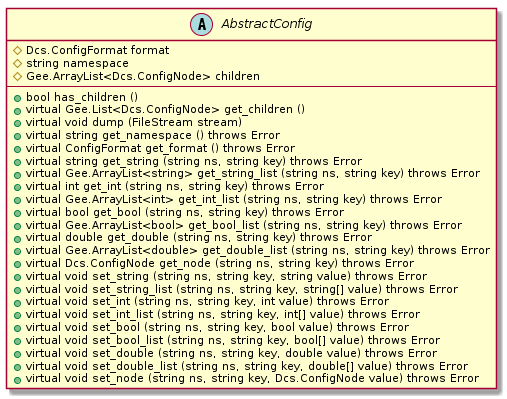
\includegraphics[width=\textwidth]{figures/design/class/core/abstract-config}
          %\caption{Class Diagram for a DcsAbstractConfig}
          \label{fig:dsg-classes-abs-config}
        \end{figure}
      \end{minipage}

      \emph{DcsApplication}

      \vspace*{-0.75cm}
      \begin{minipage}[t]{0.5\textwidth}
        \vspace*{0.5cm}
        Applications in OpenDCS are the base of services as well as GUI and CLI
        processes. Each needs to function as a Model-View-Controller (MVC)
        application in order to have a standardized architecture for plugin
        developers to connect to.
      \end{minipage} \hfill
      \begin{minipage}[t]{0.45\textwidth}
        \begin{figure}[H]
          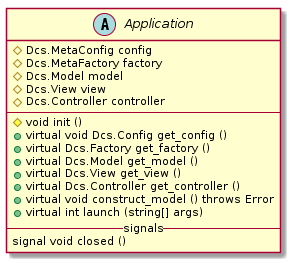
\includegraphics[width=\textwidth]{figures/design/class/core/application}
          %\caption{Class Diagram for a DcsApplication}
          \label{fig:dsg-classes-application}
        \end{figure}
      \end{minipage}

      \emph{DcsConfigNode}

      \vspace*{-0.75cm}
      \begin{minipage}[t]{0.5\textwidth}
        \vspace*{0.5cm}
        Configuration is a core concept of OpenDCS services and applications,
        and central to them is the configuration node. It relates to a single
        configuration object implemented using XML, JSON, and INI key files
        depending on how the configuration file has been implemented. These
        configuration nodes are used by factories to produce node objects which
        form the base of the data model component of the MVC application.
      \end{minipage} \hfill
      \begin{minipage}[t]{0.45\textwidth}
        \begin{figure}[H]
          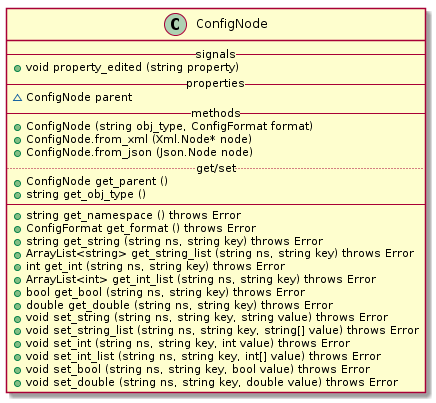
\includegraphics[width=\textwidth]{figures/design/class/core/config-node}
          %\caption{Class Diagram for a DcsConfigNode}
          \label{fig:dsg-classes-config-node}
        \end{figure}
      \end{minipage}

      \emph{DcsConfig}

      \vspace*{-0.75cm}
      \begin{minipage}[t]{0.5\textwidth}
        \vspace*{0.5cm}
        This interface is the generic type which is implemented accross other
        configuration types to provide the contract to use by the developer of
        other configuration types.
      \end{minipage} \hfill
      \begin{minipage}[t]{0.45\textwidth}
        \begin{figure}[H]
          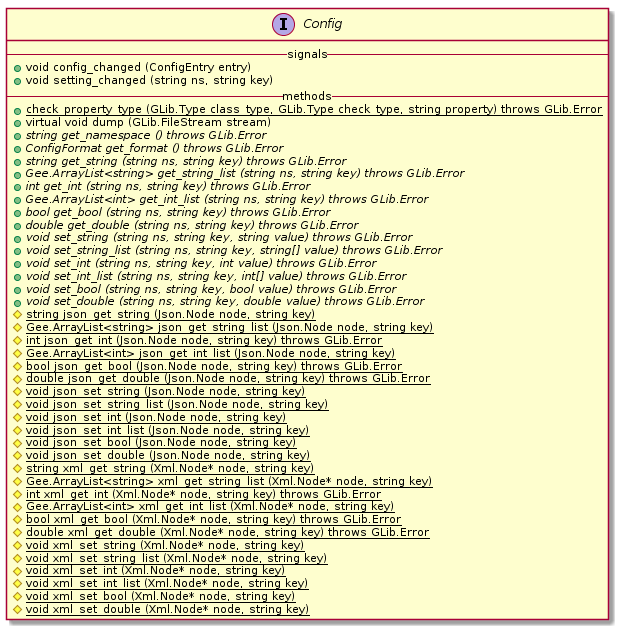
\includegraphics[width=\textwidth]{figures/design/class/core/config}
          %\caption{Class Diagram for a DcsConfig}
          \label{fig:dsg-classes-config}
        \end{figure}
      \end{minipage}

      \emph{DcsController}

      \vspace*{-0.75cm}
      \begin{minipage}[t]{0.5\textwidth}
        \vspace*{0.5cm}
        % TODO provide citation
        A controller in an MVC application is responsible for accepting input
        and converting it to commands for the model or the view.
      \end{minipage} \hfill
      \begin{minipage}[t]{0.45\textwidth}
        \begin{figure}[H]
          \includegraphics[width=\textwidth]{figures/design/class/core/controller}
          %\caption{Class Diagram for a DcsController}
          \label{fig:dsg-classes-controller}
        \end{figure}
      \end{minipage}

      \emph{DcsDataSeries}

      \vspace*{-0.75cm}
      \begin{minipage}[t]{0.5\textwidth}
        \vspace*{0.5cm}
        A data series within the context of OpenDCS is a building block for
        node objects that need to contain an array of values, some examples of
        this are a feedback controller, a chart trace, or a signal filter.
      \end{minipage} \hfill
      \begin{minipage}[t]{0.45\textwidth}
        \begin{figure}[H]
          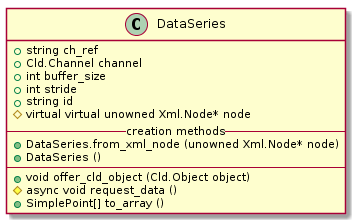
\includegraphics[width=0.6\textwidth]{figures/design/class/core/dataseries}
          %\caption{Class Diagram for a DcsDataSeries}
          \label{fig:dsg-classes-data-series}
        \end{figure}
      \end{minipage}

      \emph{DcsDBusInterface}

      \vspace*{-0.75cm}
      \begin{minipage}[t]{0.5\textwidth}
        \vspace*{0.5cm}
        In GLib applications DBus interfaces are used by services to create an
        API similar to what would be provided by a REST API. This object is
        carry over from the software that OpenDCS was forked from and will very
        likely find a home in the Net namespace in future versions.
      \end{minipage} \hfill
      \begin{minipage}[t]{0.45\textwidth}
        \begin{figure}[H]
          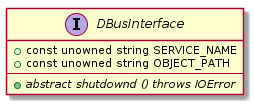
\includegraphics[width=0.8\textwidth]{figures/design/class/core/dbus-interface}
          %\caption{Class Diagram for a DcsDBusInterface}
          \label{fig:dsg-classes-dbus-interface}
        \end{figure}
      \end{minipage}

      \emph{DcsFactory}

      \vspace*{-0.75cm}
      \begin{minipage}[t]{0.5\textwidth}
        \vspace*{0.5cm}
        Factories in OpenDCS are a means to define a generic way of building
        objects from configuration nodes without having to define a construction
        method within each. It defines the requirements for others implementing
        this on how they need to consume properties and child nodes using the
        parameter specification abilities afforded by GLib objects.
      \end{minipage} \hfill
      \begin{minipage}[t]{0.45\textwidth}
        \begin{figure}[H]
          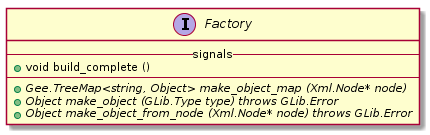
\includegraphics[width=\textwidth]{figures/design/class/core/factory}
          %\caption{Class Diagram for a DcsFactory}
          \label{fig:dsg-classes-factory}
        \end{figure}
      \end{minipage}

      \emph{DcsMessage}

      \vspace*{-0.75cm}
      \begin{minipage}[t]{0.5\textwidth}
        \vspace*{0.5cm}
        % TODO move to Net
        Messages are a serialized format of an object, or grouping of objects,
        that will be pushed and popped on message queues that are used by
        services to communicate with each other.
      \end{minipage} \hfill
      \begin{minipage}[t]{0.45\textwidth}
        \begin{figure}[H]
          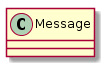
\includegraphics[width=\textwidth]{figures/design/class/core/message}
          %\caption{Class Diagram for a DcsMessage}
          \label{fig:dsg-classes-message}
        \end{figure}
      \end{minipage}

      \emph{DcsMetaConfig}

      \vspace*{-0.75cm}
      \begin{minipage}[t]{0.5\textwidth}
        \vspace*{0.5cm}
        The meta configuration class provides applications a method of loading
        multiple configurations of various types in at runtime without knowing
        exactly what they provide. It is essentially a list of configuration
        types and methods to iterate over those to get and set objects and
        properties that they provide.
      \end{minipage} \hfill
      \begin{minipage}[t]{0.45\textwidth}
        \begin{figure}[H]
          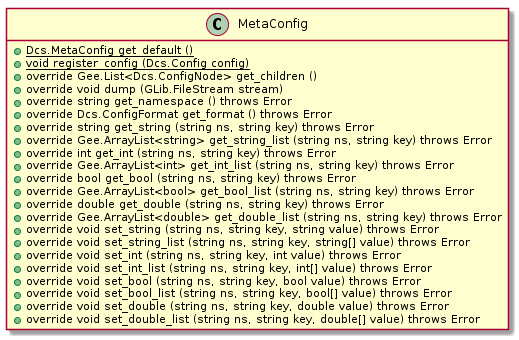
\includegraphics[width=\textwidth]{figures/design/class/core/meta-config}
          %\caption{Class Diagram for a DcsMetaConfig}
          \label{fig:dsg-classes-meta-config}
        \end{figure}
      \end{minipage}

      \emph{DcsMetaFactory}

      \vspace*{-0.75cm}
      \begin{minipage}[t]{0.5\textwidth}
        \vspace*{0.5cm}
        The meta factory class provides applications a method of loading
        multiple object factories of various types in a runtime without knowing
        what the produce for a given configuration node. It is a list of factory
        types and methods to iterate over those to be used to create object
        nodes that end up in an application's data model.
      \end{minipage} \hfill
      \begin{minipage}[t]{0.45\textwidth}
        \begin{figure}[H]
          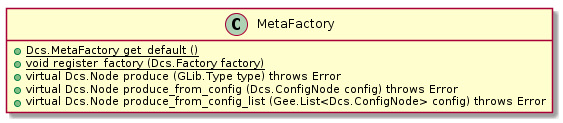
\includegraphics[width=\textwidth]{figures/design/class/core/meta-factory}
          %\caption{Class Diagram for a DcsMetaFactory}
          \label{fig:dsg-classes-meta-factory}
        \end{figure}
      \end{minipage}

      \emph{DcsModel}

      \vspace*{-0.75cm}
      \begin{minipage}[t]{0.5\textwidth}
        \vspace*{0.5cm}
        % TODO provide citation
        A model in an MVC application stores data that is retrieved using
        commands from the controller and to update what is displayed in the
        view.
      \end{minipage} \hfill
      \begin{minipage}[t]{0.45\textwidth}
        \begin{figure}[H]
          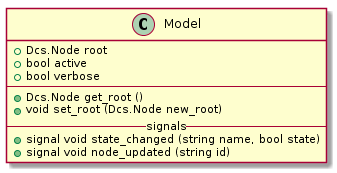
\includegraphics[width=\textwidth]{figures/design/class/core/model}
          %\caption{Class Diagram for a DcsModel}
          \label{fig:dsg-classes-model}
        \end{figure}
      \end{minipage}

      \emph{DcsNode}

      \vspace*{-0.75cm}
      \begin{minipage}[t]{0.5\textwidth}
        \vspace*{0.5cm}
        The node class is a fundamental component of constructing the data model
        for services, it is extends a tree map ADT and is meant to contain other
        objects that derive it. Nodes have properties, an optional parent, and
        optional children, all of which describe the object and allow it to be
        constructed generically and placed within the data model tree.
      \end{minipage} \hfill
      \begin{minipage}[t]{0.45\textwidth}
        \begin{figure}[H]
          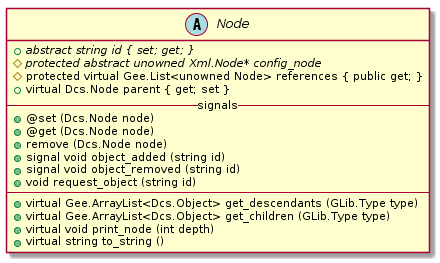
\includegraphics[width=\textwidth]{figures/design/class/core/node}
          %\caption{Class Diagram for a DcsNode}
          \label{fig:dsg-classes-node}
        \end{figure}
      \end{minipage}

      \emph{DcsObject}

      \vspace*{-0.75cm}
      \begin{minipage}[t]{0.5\textwidth}
        \vspace*{0.5cm}
        An object is the base interface for all classes to implement that work
        across OpenDCS libraries and within service data models.
      \end{minipage} \hfill
      \begin{minipage}[t]{0.45\textwidth}
        \begin{figure}[H]
          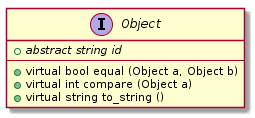
\includegraphics[width=0.8\textwidth]{figures/design/class/core/object}
          %\caption{Class Diagram for a DcsObject}
          \label{fig:dsg-classes-object}
        \end{figure}
      \end{minipage}

      \emph{DcsPluginInformation}

      \vspace*{-0.75cm}
      \begin{minipage}[t]{0.5\textwidth}
        \vspace*{0.5cm}
        The plugin information class will be used to describe features that the
        plugin provides, for example if a plugin is meant to read values from a
        piece of data acquisition hardware it will provide the values read as
        analog input channels.
      \end{minipage} \hfill
      \begin{minipage}[t]{0.45\textwidth}
        \begin{figure}[H]
          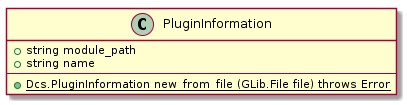
\includegraphics[width=\textwidth]{figures/design/class/core/plugin-information}
          %\caption{Class Diagram for a DcsPluginInformation}
          \label{fig:dsg-classes-plugin-information}
        \end{figure}
      \end{minipage}

      \emph{DcsPluginManager}

      \vspace*{-0.75cm}
      \begin{minipage}[t]{0.5\textwidth}
        \vspace*{0.5cm}
        In other namespaces plugin managers will use this common class so that
        services have a general base for the functionality the plugin system is
        meant to provide.
      \end{minipage} \hfill
      \begin{minipage}[t]{0.45\textwidth}
        \begin{figure}[H]
          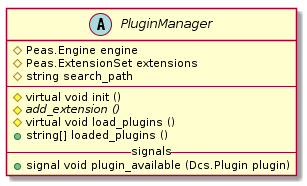
\includegraphics[width=\textwidth]{figures/design/class/core/plugin-manager}
          %\caption{Class Diagram for a DcsPluginManager}
          \label{fig:dsg-classes-plugin-manager}
        \end{figure}
      \end{minipage}

      \emph{DcsPlugin}

      \vspace*{-0.75cm}
      \begin{minipage}[t]{0.5\textwidth}
        \vspace*{0.5cm}
        A plugin object is the class that other plugin types base off of, it
        defines the basic requirements that libpeas has of plugin extensions.
        All plugins in OpenDCS will additionally have the ability to perform
        some execution in a thread, so the provision for that has been added.
      \end{minipage} \hfill
      \begin{minipage}[t]{0.45\textwidth}
        \begin{figure}[H]
          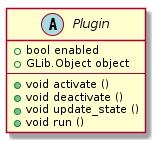
\includegraphics[width=0.5\textwidth]{figures/design/class/core/plugin}
          %\caption{Class Diagram for a DcsPlugin}
          \label{fig:dsg-classes-plugin}
        \end{figure}
      \end{minipage}

      \emph{Point}

      \vspace*{-0.75cm}
      \begin{minipage}[t]{0.5\textwidth}
        \vspace*{0.5cm}
        Points are a simple class that are used at a variety of locations
        including in measurements, data series value groups, and chart traces
        in the GUI which hasn't been included in this report.
      \end{minipage} \hfill
      \begin{minipage}[t]{0.45\textwidth}
        \begin{figure}[H]
          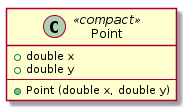
\includegraphics[width=0.6\textwidth]{figures/design/class/core/point}
          %\caption{Class Diagram for a DcsPoint}
          \label{fig:dsg-classes-point}
        \end{figure}
      \end{minipage}

      \emph{DcsRefContainer}

      \vspace*{-0.75cm}
      \begin{minipage}[t]{0.5\textwidth}
        \vspace*{0.5cm}
        References are an integral part of how the objects contained in a data
        model connect to each other, this class provides the ability to work
        with those references in a safe manner.
      \end{minipage} \hfill
      \begin{minipage}[t]{0.45\textwidth}
        \begin{figure}[H]
          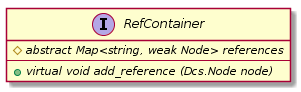
\includegraphics[width=\textwidth]{figures/design/class/core/ref-container}
          %\caption{Class Diagram for a DcsRefContainer}
          \label{fig:dsg-classes-ref-container}
        \end{figure}
      \end{minipage}

      \emph{DcsRefLinker}

      \vspace*{-0.75cm}
      \begin{minipage}[t]{0.5\textwidth}
        \vspace*{0.5cm}
        Reference linking is performed by an application after every time new
        references have been added to an object. This object uses the singleton
        pattern as it contains data about the entire application and would
        present problems if multiple instances existed.
      \end{minipage} \hfill
      \begin{minipage}[t]{0.45\textwidth}
        \begin{figure}[H]
          \includegraphics[width=\textwidth]{figures/design/class/core/ref-linker}
          %\caption{Class Diagram for a DcsRefLinker}
          \label{fig:dsg-classes-ref-linker}
        \end{figure}
      \end{minipage}

      \emph{DcsSerializable}

      \vspace*{-0.75cm}
      \begin{minipage}[t]{0.5\textwidth}
        \vspace*{0.5cm}
        This interface is used by objects that will need to be serialized and
        deserialized for the purpose of passing across networks using ZeroMQ and
        REST messaging.
      \end{minipage} \hfill
      \begin{minipage}[t]{0.45\textwidth}
        \begin{figure}[H]
          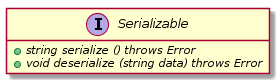
\includegraphics[width=0.8\textwidth]{figures/design/class/core/serializable}
          %\caption{Class Diagram for a DcsSerializable}
          \label{fig:dsg-classes-serializable}
        \end{figure}
      \end{minipage}

      \emph{DcsSyslog}

      \vspace*{-0.75cm}
      \begin{minipage}[t]{0.5\textwidth}
        \vspace*{0.5cm}
        The logging facility provides a format for output strings and controls
        what level of messages will be output based on a variable controlling
        verbosity. It provides control to the user over the output depending on
        whether they want to see minimal messages all the way up to very
        verbose debugging and trace messages.
      \end{minipage} \hfill
      \begin{minipage}[t]{0.45\textwidth}
        \begin{figure}[H]
          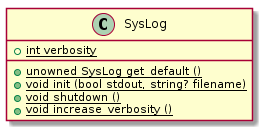
\includegraphics[width=0.8\textwidth]{figures/design/class/core/syslog}
          %\caption{Class Diagram for a DcsSyslog}
          \label{fig:dsg-classes-syslog}
        \end{figure}
      \end{minipage}

      \emph{DcsView}

      \vspace*{-0.75cm}
      \begin{minipage}[t]{0.5\textwidth}
        \vspace*{0.5cm}
        A view in an MVC application is used to generate new output based on
        changes to the model.
      \end{minipage} \hfill
      \begin{minipage}[t]{0.45\textwidth}
        \begin{figure}[H]
          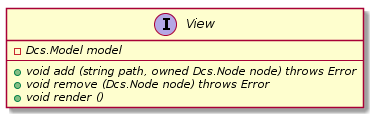
\includegraphics[width=\textwidth]{figures/design/class/core/view}
          %\caption{Class Diagram for a DcsView}
          \label{fig:dsg-classes-view}
        \end{figure}
      \end{minipage}

    \newpage

    \subsubsection{Data Acquisition Library}\label{sec:dsg-classes-daq}

      Classes in the DAQ library will provide the functionality required to
      create objects that communicate with physical devices. Plugins in this
      namespace are referred to as devices, these device plugins are meant to be
      created to read and write real world values and present them over the
      message queueing systems available.

      \emph{DcsDaqDeviceManager}

      \vspace*{-0.75cm}
      \begin{minipage}[t]{0.5\textwidth}
        \vspace*{0.5cm}
        The device manager class is the DAQ namespace specific implementation of
        the plugin manager to be used by services and applications that want to
        load hardware device type plugins.
      \end{minipage} \hfill
      \begin{minipage}[t]{0.45\textwidth}
        \begin{figure}[H]
          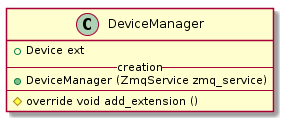
\includegraphics[width=0.8\textwidth]{figures/design/class/daq/device-manager}
          %\caption{Class Diagram for a DcsDaqDeviceManager}
          \label{fig:dsg-classes-daq-device-manager}
        \end{figure}
      \end{minipage}

      \emph{DcsDaqDevice}

      \vspace*{-0.75cm}
      \begin{minipage}[t]{0.5\textwidth}
        \vspace*{0.5cm}
        This serves as a base for any device plugins that will be developed and
        loaded by services and applications that contain a device manager.
      \end{minipage} \hfill
      \begin{minipage}[t]{0.45\textwidth}
        \begin{figure}[H]
          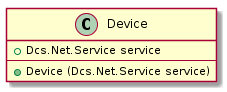
\includegraphics[width=0.6\textwidth]{figures/design/class/daq/device}
          %\caption{Class Diagram for a DcsDaqDevice}
          \label{fig:dsg-classes-daq-device}
        \end{figure}
      \end{minipage}

      \emph{DcsDaqFactory}

      \vspace*{-0.75cm}
      \begin{minipage}[t]{0.5\textwidth}
        \vspace*{0.5cm}
        The factory class in this namespace serves the same function as other
        factories, except that it produces DAQ specific objects. It is meant to
        be used with the DcsMetaFactory class as part of a larger application.
      \end{minipage} \hfill
      \begin{minipage}[t]{0.45\textwidth}
        \begin{figure}[H]
          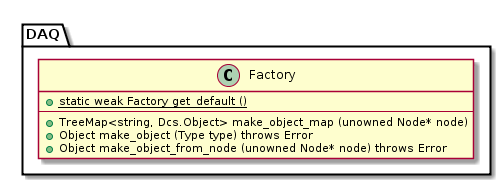
\includegraphics[width=\textwidth]{figures/design/class/daq/factory}
          %\caption{Class Diagram for a DcsDaqFactory}
          \label{fig:dsg-classes-daq-factory}
        \end{figure}
      \end{minipage}

    \subsubsection{Data Logging Library}\label{sec:dsg-classes-log}

      Classes in the data logging library will provide the functionality
      required to read and write data values that it has received into any
      format that has been defined by the plugins. Plugins in this namespace are
      referred to as backends, these logging plugins are meant to create and
      work with different file formats, databases, and whatever else makes sense
      to record data onto.

      \emph{DcsLogBackendManager}

      \vspace*{-0.75cm}
      \begin{minipage}[t]{0.5\textwidth}
        \vspace*{0.5cm}
        The backend manager class is the Log namespace specific implementation
        of the plugin manager to be used by services and applications that want
        to load logging backend type plugins.
      \end{minipage} \hfill
      \begin{minipage}[t]{0.45\textwidth}
        \begin{figure}[H]
          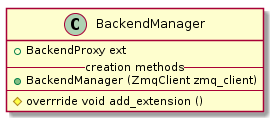
\includegraphics[width=0.8\textwidth]{figures/design/class/log/backend-manager}
          %\caption{Class Diagram for a DcsLogBackendManager}
          \label{fig:dsg-classes-log-backend-manager}
        \end{figure}
      \end{minipage}

      \emph{DcsLogBackend}

      \vspace*{-0.75cm}
      \begin{minipage}[t]{0.5\textwidth}
        \vspace*{0.5cm}
        This serves as a base for any backend plugin that will be developed and
        loaded by services and applications that contain a backend manager.
      \end{minipage} \hfill
      \begin{minipage}[t]{0.45\textwidth}
        \begin{figure}[H]
          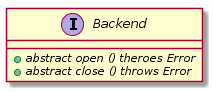
\includegraphics[width=0.6\textwidth]{figures/design/class/log/backend}
          %\caption{Class Diagram for a DcsLogBackend}
          \label{fig:dsg-classes-log-backend}
        \end{figure}
      \end{minipage}

      \emph{DcsLogFactory}

      \vspace*{-0.75cm}
      \begin{minipage}[t]{0.5\textwidth}
        \vspace*{0.5cm}
        The factory class in this namespace serves the same function as other
        factories, except that it produces Log specific objects. It is meant to
        be used with the DcsMetaFactory class as part of a larger application.
      \end{minipage} \hfill
      \begin{minipage}[t]{0.45\textwidth}
        \begin{figure}[H]
          \includegraphics[width=\textwidth]{figures/design/class/log/factory}
          %\caption{Class Diagram for a DcsLogFactory}
          \label{fig:dsg-classes-log-factory}
        \end{figure}
      \end{minipage}

    \subsubsection{Feedback Control Library}\label{sec:dsg-classes-ctl}

      Classes in the feedback control library will provide the functionality
      required to
      read and write data values that it has received into any
      format that has been defined by the plugins. Plugins in this namespace are
      referred to as backends, these logging plugins are meant to create and
      work with different file formats, databases, and whatever else makes sense
      to record data onto

      \emph{DcsControlControllerManager}

      \vspace*{-0.75cm}
      \begin{minipage}[t]{0.5\textwidth}
        \vspace*{0.5cm}
        The controller manager class is the Control namespace specific
        implementation of the plugin manager to be used by services and
        applications that want to load feedback controller type plugins.
      \end{minipage} \hfill
      \begin{minipage}[t]{0.45\textwidth}
        \begin{figure}[H]
          \includegraphics[width=0.8\textwidth]{figures/design/class/control/controller-manager}
          \label{fig:dsg-classes-control-controller-manager}
        \end{figure}
      \end{minipage}

      \emph{DcsControlController}

      \vspace*{-0.75cm}
      \begin{minipage}[t]{0.5\textwidth}
        \vspace*{0.5cm}
        This serves as a base for any controller plugin that will be developed
        and loaded by services and applications that contain a controller
        manager.
      \end{minipage} \hfill
      \begin{minipage}[t]{0.45\textwidth}
        \begin{figure}[H]
          \includegraphics[width=0.6\textwidth]{figures/design/class/control/controller}
          \label{fig:dsg-classes-control-controller}
        \end{figure}
      \end{minipage}

      \emph{DcsControlFactory}

      \vspace*{-0.75cm}
      \begin{minipage}[t]{0.5\textwidth}
        \vspace*{0.5cm}
        The factory class in this namespace serves the same function as other
        factories, except that it produces Control specific objects. It is
        meant to be used with the DcsMetaFactory class as part of a larger
        application.
      \end{minipage} \hfill
      \begin{minipage}[t]{0.45\textwidth}
        \begin{figure}[H]
          \includegraphics[width=\textwidth]{figures/design/class/control/factory}
          \label{fig:dsg-classes-control-factory}
        \end{figure}
      \end{minipage}

    \newpage

    \subsubsection{Networking Library}\label{sec:dsg-classes-net}

      The networking library contains classes that are used to communicate with
      other services. This ability is accomplished using ZeroMQ and REST as the
      messaging systems, but is left open for others such as DBus or RabbitMQ.

      \emph{DcsNetFactory}

      \vspace*{-0.75cm}
      \begin{minipage}[t]{0.5\textwidth}
        \vspace*{0.5cm}
        The factory class in this namespace serves the same function as other
        factories, except that it produces Net specific objects. It is meant to
        be used with the DcsMetaFactory class as part of a larger application.
      \end{minipage} \hfill
      \begin{minipage}[t]{0.45\textwidth}
        \begin{figure}[H]
          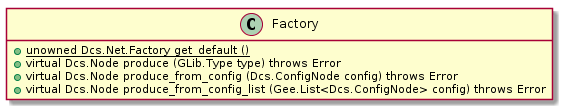
\includegraphics[width=\textwidth]{figures/design/class/net/factory}
          %\caption{Class Diagram for a DcsNetFactory}
          \label{fig:dsg-classes-net-factory}
        \end{figure}
      \end{minipage}

      \emph{DcsNetService}

      \vspace*{-0.75cm}
      \begin{minipage}[t]{0.5\textwidth}
        \vspace*{0.5cm}
        Services are an extension of applications and use the same MVC design
        pattern, but they add the concept of plugin systems and expose features
        that are required by plugins to function as part of the system.
      \end{minipage} \hfill
      \begin{minipage}[t]{0.45\textwidth}
        \begin{figure}[H]
          \includegraphics[width=\textwidth]{figures/design/class/net/service}
          %\caption{Class Diagram for a DcsNetService}
          \label{fig:dsg-classes-net-service}
        \end{figure}
      \end{minipage}

      \emph{DcsNetRestService}

      \vspace*{-0.75cm}
      \begin{minipage}[t]{0.5\textwidth}
        \vspace*{0.5cm}
        This is an abstract base that service implementations must extend and
        define if they want to provide a RESTful API. It exists mainly to be
        added as a contract to the DcsNetService class to ensure services
        include one.
      \end{minipage} \hfill
      \begin{minipage}[t]{0.45\textwidth}
        \begin{figure}[H]
          \includegraphics[width=0.8\textwidth]{figures/design/class/net/rest-service}
          %\caption{Class Diagram for a DcsNetRestService}
          \label{fig:dsg-classes-net-rest-service}
        \end{figure}
      \end{minipage}

      \emph{DcsNetPublish}

      \vspace*{-0.75cm}
      \begin{minipage}[t]{0.5\textwidth}
        \vspace*{0.5cm}
        A publish object makes a connection to a ZeroMQ context and provides a
        means of configuring this type of socket using the configuration and
        production methods of this project.
      \end{minipage} \hfill
      \begin{minipage}[t]{0.45\textwidth}
        \begin{figure}[H]
          \includegraphics[width=0.8\textwidth]{figures/design/class/net/publish}
          %\caption{Class Diagram for a DcsNetPublish}
          \label{fig:dsg-classes-net-publish}
        \end{figure}
      \end{minipage}

      \emph{DcsNetSubscribe}

      \vspace*{-0.75cm}
      \begin{minipage}[t]{0.5\textwidth}
        \vspace*{0.5cm}
        A subscribe object makes a connection to a ZeroMQ context and provides a
        means of configuring this type of socket using the configuration and
        production methods of this project.
      \end{minipage} \hfill
      \begin{minipage}[t]{0.45\textwidth}
        \begin{figure}[H]
          \includegraphics[width=\textwidth]{figures/design/class/net/subscribe}
          %\caption{Class Diagram for a DcsNetSubscribe}
          \label{fig:dsg-classes-net-subscribe}
        \end{figure}
      \end{minipage}

      \emph{DcsNetRequest}

      \vspace*{-0.75cm}
      \begin{minipage}[t]{0.5\textwidth}
        \vspace*{0.5cm}
        A request object makes a connection to a ZeroMQ context and provides a
        means of configuring this type of socket using the configuration and
        production methods of this project.
      \end{minipage} \hfill
      \begin{minipage}[t]{0.45\textwidth}
        \begin{figure}[H]
          \includegraphics[width=0.8\textwidth]{figures/design/class/net/request}
          %\caption{Class Diagram for a DcsNetRequest}
          \label{fig:dsg-classes-net-request}
        \end{figure}
      \end{minipage}

      \emph{DcsNetReply}

      \vspace*{-0.75cm}
      \begin{minipage}[t]{0.5\textwidth}
        \vspace*{0.5cm}
        A reply object makes a connection to a ZeroMQ context and provides a
        means of configuring this type of socket using the configuration and
        production methods of this project.
      \end{minipage} \hfill
      \begin{minipage}[t]{0.45\textwidth}
        \begin{figure}[H]
          \includegraphics[width=0.8\textwidth]{figures/design/class/net/reply}
          %\caption{Class Diagram for a DcsNetReply}
          \label{fig:dsg-classes-net-reply}
        \end{figure}
      \end{minipage}

  \newpage

  \subsection{Class Diagrams}\label{sec:dsg-class-dia}

    Using the objects defined in Section~\ref{sec:dsg-classes} this section will
    define the structure of the core components of how the services will be
    constructed. These consist of configurations, object factories to produce
    generic objects using configuration nodes, plugins, and services or
    applications.

    \emph{Configuration Composition}

    OpenDCS services are based on a concept of being configurable at many
    levels, the diagram provided for the service configuration composition
    in Figure~\ref{fig:dsg-class-config} shows how the constituent
    classes are organized. At the top level the service contains a single
    configuration class \emph{Dcs.MetaConfig} that itself contains all of
    the other configurations regardless of type and it is used by the
    service as a single point into the group. This design allows for
    a variety of configuration concepts including variables set during
    launch using command line arguments, files loaded from the system,
    and partial configuration files loaded by the plugins during setup.

    \begin{figure}[H]
      \includegraphics[width=\textwidth]{figures/design/class/config}
      \caption{Class Diagram for the Configuration Composition}
      \label{fig:dsg-class-config}
    \end{figure}

    \emph{Object Factory Composition}

    Much like the configuration concept, the services have a single point for
    application access which is shown in Figure~\ref{fig:dsg-class-factory}.
    With this component the factories consume \emph{Dcs.ConfigNode} objects
    and produce \emph{Dcs.Node} objects which form the data model that is used
    by the entire service or application. It is meant to do this in a very
    generic fashion where each namespace is responsible for providing the
    objects that they know of, as well as a method to allow plugins which are
    completely unknown to the service the ability to construct new objects that
    will integrate with the system.

    \begin{figure}[H]
      \includegraphics[width=\textwidth]{figures/design/class/factory}
      \caption{Class Diagram for the Object Factory Composition}
      \label{fig:dsg-class-factory}
    \end{figure}

    \emph{Plugin System Composition}

    The plugin system is the next fundamental component of the design and in
    it the idea is to have each namespace define a manager and plugins of their
    own type, these are then used with any service that wants to implement that
    form of plugin. While this could have been implemented as a single plugin
    manager and plugin type this is intended to allow for a more logical means
    of installing and managing plugins when installed on a host. Core to these
    plugins is the ability to access the service application and what it
    provides, and more specifically the model, view, and controller (MVC) of
    that process. Having access to the MVC means that the plugin can attach new
    objects to the data model providing they follow the standard format, to add
    new view components that are rendered to an end user, and to communicate
    with the abilities of the service through the controller.

    \begin{figure}[H]
      \includegraphics[width=\textwidth]{figures/design/class/plugin}
      \caption{Class Diagram for the Plugin System Composition}
      \label{fig:dsg-class-plugin}
    \end{figure}

    \emph{Service/Application Composition}

    Services, or applications, are the final piece that bring together the
    other concepts presented in this section. They are responsible for loading
    all plugins during launch, reading and combining all configurations,
    producing the data model using the aggregated object factories, and
    providing the plugins with what they require to put messages onto the
    message queues of the service that are wired up with other services.

    \begin{figure}[H]
        \includegraphics[width=\textwidth]{figures/design/class/service}
      \caption{Class Diagram for the Service/Application Composition}
      \label{fig:dsg-class-service}
    \end{figure}

    \emph{Complete Class Diagram for the Entire Project}

    The complete class diagram for OpenDCS would not fit onto a single page, or
    spanning multiple pages, in any way that would make it useful to the
    reader.  As that is the case the file has been provided on the disc that
    the report has been submitted on at the path \\
    \texttt{documents/report/figures/design/class/opendcs.png}. Alternatively,
    this file can be retrieved from the GitHub repository where the files used
    to create this report reside at \url{https://github.com/open-dcs/doc/blob/master/report/figures/design/class/opendcs.png}.

  \newpage

  \subsection{Sequence Diagrams}\label{sec:dsg-sequence}

    The project life cycle sequence does not impact the development of this
    software, but it is important to the client that they understand how it
    would affect their workflow. Figure~\ref{fig:dsg-sequence-life-cycle} shows
    a proposed method without getting into the specifics of configuration. As
    that is a somewhat complicated task that requires knowledge of the system as
    well the configuration language used, XML and JSON, it would take
    significant effort to adequately describe and is outside of the scope of
    this document.

    \begin{figure}[H]
      \includegraphics[width=0.8\textwidth,center]{figures/design/sequence/project-lifecycle}
      \caption{Project Life Cycle Sequence Diagram}
      \label{fig:dsg-sequence-life-cycle}
    \end{figure}

    \newpage

    All of the services that will be developed as part of OpenDCS rely heavily
    on the usage of plugins, as such it is worthwhile to outline how the generic
    service concept will go about loading plugins from the file system. What is
    not described in Figure~\ref{fig:dsg-sequence-load-plugins} is how to create
    a plugin, or where the system expects them to reside. This information will
    be given later on in Section~\ref{sec:inst}.

    \begin{figure}[H]
      \includegraphics[width=0.8\textwidth,center]{figures/design/sequence/load-plugins}
      \caption{Plugin Loading Sequence Diagram}
      \label{fig:dsg-sequence-load-plugins}
    \end{figure}

    The next three sequence diagrams show the process sequence of key concepts.
    Figure~\ref{fig:dsg-sequence-measure-request} is meant to describe what
    should happen when a user of the system requests a measurement from the DAQ
    service, Figure~\ref{fig:dsg-sequence-query-request} for a data query of
    the logging service, and Figure~\ref{fig:dsg-sequence-control-request} for
    a process control change of the feedback control service.

    \newpage

    A measurement in OpenDCS is performed by a device plugin, the DAQ service
    itself is only responsible for loading the plugin and providing the
    connection between the device and the messaging system that other services
    and applications communicate to it through. In the case of a request-reply
    type request made by the end user where a measurement is requested and the
    measured value is provided in a reply the sequence follows this pattern.

    \begin{figure}[H]
      \includegraphics[width=\textwidth]{figures/design/sequence/measure-request}
      \caption{Data Acquisition Service Measurement Sequence Diagram}
      \label{fig:dsg-sequence-measure-request}
    \end{figure}

    Logging services, like the DAQ service, do the bulk of the actual work
    through plugins that communicate with underlying files and databases
    depending on what they've been developed to use. The pattern used by users
    of the service always follow a request-reply sequence where the user acting
    on the service makes a query request that defines a date and time range that
    they are interested in and the service provides the result as a formatted
    data set.

    \begin{figure}[H]
      \includegraphics[width=\textwidth]{figures/design/sequence/query-request}
      \caption{Data Log Service Query Sequence Diagram}
      \label{fig:dsg-sequence-query-request}
    \end{figure}

    Lastly, the feedback control service, again like the DAQ service, does its
    work using plugins that receive data from the DAQ service, perform and
    calculation in a controller plugin and feed the change back to the DAQ
    service to perform the actual work. The sequence given here is that of a
    single change request being made by the user, in reality the interaction
    between the control and DAQ services would take place several times and
    would not necessarily be done over a request-reply socket pair, but for
    brevity this is how it's been illustrated.

    \begin{figure}[H]
      \includegraphics[width=\textwidth]{figures/design/sequence/control-request}
      \caption{Feedback Controller Service Change Sequence Diagram}
      \label{fig:dsg-sequence-control-request}
    \end{figure}

  \newpage

  \subsection{Component Diagrams}\label{sec:dsg-component}

    OpenDCS is a service oriented architecture where each should be developed to
    very similar to the others. The standard component format is shown in
    Figure~\ref{fig:dsg-component-service}, this provides a very high level
    outline of the intended way for a service to be constructed to provide a way
    for external applications to communicate with it.

    \begin{figure}[H]
      \includegraphics[width=0.6\textwidth,center]{figures/design/component/service}
      \caption{Service Component Diagram}
      \label{fig:dsg-component-service}
    \end{figure}

    Additionally, the services will all be designed to implement a plugin
    manager system so that a common framework for plugins can be utilized. This
    framework is given in Figure~\ref{fig:dsg-component-plugin} which
    illustrates how plugins are loaded and what they should provide. The term
    ``Meta'' is used to describe that the configuration and factory components
    of services are constructed of multiples of the same type across the various
    namespaces.

    \begin{figure}[H]
      \includegraphics[width=0.6\textwidth,center]{figures/design/component/plugin}
      \caption{Plugin Component Diagram}
      \label{fig:dsg-component-plugin}
    \end{figure}


  \newpage
  \section{Development}\label{sec:dev}

  \subsection{Autotools Build Systems}\label{sec:dev-ac}

  \subsection{REST APIs}\label{sec:rest}

    A high level overview of the RESTful APIs provided by the services is given
    here, these add a method of interoperability among these and other web
    services that want to communicate with them. In most cases this means using
    the common HTTP verbs GET, POST, PUT, and DELETE as operations.

    \subsubsection{Common to All Services}\label{sec:rest-common}

      This section describes the common APIs for services that contain
      networking objects. Each service with have dedicated publishing,
      subscribing, requesting, and replying sockets where necessary to function
      as intended but they will also be capable of having additional socket
      types configured at runtime to add functionality and leave future options
      open for concepts like proxies and brokers.

      \large{\textbf{Publishers}}

      \begin{table}[H]
        \centering
        \begin{tabular}{p{8cm} p{10cm}}
          \toprule
          \emph{Resource} & \emph{Description} \\ [0.5ex]
          \midrule
          GET /api/net/publishers & List all publishers \\
          GET /api/net/publishers/:id & Show a publisher \\
          POST /api/net/publishers/:id & Add a publisher \\
          PUT /api/net/publishers/:id & Update a publisher \\
          DELETE /api/net/publishers/:id & Remove a publisher \\
          \bottomrule
        \end{tabular}
        \caption{API for the Publishers in Services}\label{tab:rest-common-pub}
      \end{table}

      \large{\textbf{Subscribers}}

      \begin{table}[H]
        \centering
        \begin{tabular}{p{8cm} p{10cm}}
          \toprule
          \emph{Resource} & \emph{Description} \\ [0.5ex]
          \midrule
          GET /api/net/subscribers & List all subscriber \\
          GET /api/net/subscribers/:id & Show a subscriber \\
          POST /api/net/subscribers/:id & Add a subscriber \\
          PUT /api/net/subscribers/:id & Update a subscriber \\
          DELETE /api/net/subscribers/:id & Remove a subscriber \\
          \bottomrule
        \end{tabular}
        \caption{API for the Subscribers in Services}\label{tab:rest-common-sub}
      \end{table}

      \large{\textbf{Requesters}}

      \begin{table}[H]
        \centering
        \begin{tabular}{p{8cm} p{10cm}}
          \toprule
          \emph{Resource} & \emph{Description} \\ [0.5ex]
          \midrule
          GET /api/net/requesters & List all requesters \\
          GET /api/net/requesters/:id & Show a requester \\
          POST /api/net/requesters/:id & Add a requester \\
          PUT /api/net/requesters/:id & Update a requester \\
          DELETE /api/net/requesters/:id & Remove a requester \\
          \bottomrule
        \end{tabular}
        \caption{API for the Requesters in Services}\label{tab:rest-common-req}
      \end{table}

      \large{\textbf{Repliers}}

      \begin{table}[H]
        \centering
        \begin{tabular}{p{8cm} p{10cm}}
          \toprule
          \emph{Resource} & \emph{Description} \\ [0.5ex]
          \midrule
          GET /api/net/repliers & List all repliers \\
          GET /api/net/repliers/:id & Show a replier \\
          POST /api/net/repliers/:id & Add a replier \\
          PUT /api/net/repliers/:id & Update a replier \\
          DELETE /api/net/repliers/:id & Remove a replier \\
          \bottomrule
        \end{tabular}
        \caption{API for the Repliers in Services}\label{tab:rest-common-rep}
      \end{table}

    \subsubsection{Data Acquisition Service}\label{sec:rest-daq}

      \large{\textbf{Devices}}

      \begin{table}[H]
        \centering
        \begin{tabular}{p{8cm} p{10cm}}
          \toprule
          \emph{Resource} & \emph{Description} \\ [0.5ex]
          \midrule
          GET /api/daq/devices & List all devices \\
          GET /api/daq/devices/enabled & List all enabled devices \\
          GET /api/daq/devices/:id & Show a device \\
          POST /api/daq/devices/:id & Enable a device \\
          PUT /api/daq/devices/:id & Update a device \\
          DELETE /api/daq/devices/:id & Disable a device \\
          \bottomrule
        \end{tabular}
        \caption{API for the DAQ Service Devices}\label{tab:rest-daq-dev}
      \end{table}

      \large{\textbf{Sensors}}

      \begin{table}[H]
        \centering
        \begin{tabular}{p{8cm} p{10cm}}
          \toprule
          \emph{Resource} & \emph{Description} \\ [0.5ex]
          \midrule
          GET /api/daq/sensors & List all sensors \\
          GET /api/daq/sensors/:id & Show a sensor \\
          POST /api/daq/sensors/:id & Add a sensor \\
          PUT /api/daq/sensors/:id & Update a sensor \\
          DELETE /api/daq/sensors/:id & Remove a sensor \\
          \bottomrule
        \end{tabular}
        \caption{API for the DAQ Service Sensors}\label{tab:rest-daq-sensor}
      \end{table}

      \large{\textbf{Signals}}

      \begin{table}[H]
        \centering
        \begin{tabular}{p{8cm} p{10cm}}
          \toprule
          \emph{Resource} & \emph{Description} \\ [0.5ex]
          \midrule
          GET /api/daq/signals & List all signals \\
          GET /api/daq/signals/:id & Show a signal \\
          POST /api/daq/signals/:id & Add a signal \\
          PUT /api/daq/signals/:id & Update a signal \\
          DELETE /api/daq/signals/:id & Remove signal \\
          \bottomrule
        \end{tabular}
        \caption{API for the DAQ Service Signals}\label{tab:rest-daq-signal}
      \end{table}

      \large{\textbf{Ports}}

      \begin{table}[H]
        \centering
        \begin{tabular}{p{8cm} p{10cm}}
          \toprule
          \emph{Resource} & \emph{Description} \\ [0.5ex]
          \midrule
          GET /api/daq/ports & List all ports \\
          GET /api/daq/ports/:id & Show a port \\
          POST /api/daq/ports/:id & Add a port \\
          PUT /api/daq/ports/:id & Update a port \\
          DELETE /api/daq/ports/:id & Remove a port \\
          \bottomrule
        \end{tabular}
        \caption{API for the DAQ Service Ports}\label{tab:rest-daq-port}
      \end{table}

    \subsubsection{Data Logging Service}\label{sec:rest-log}

      \large{\textbf{Backends}}

      \begin{table}[H]
        \centering
        \begin{tabular}{p{8cm} p{10cm}}
          \toprule
          \emph{Resource} & \emph{Description} \\ [0.5ex]
          \midrule
          GET /api/log/backends & List all backends \\
          GET /api/log/backends/:id & Show a backend \\
          POST /api/log/backends/:id & Enable a backend \\
          PUT /api/log/backends/:id & Update a backend \\
          DELETE /api/log/backends/:id & Disable a backend \\
          \bottomrule
        \end{tabular}
        \caption{API for the Log Service Backends}\label{tab:rest-log-backend}
      \end{table}

      \large{\textbf{Logs}}

      \begin{table}[H]
        \centering
        \begin{tabular}{p{8cm} p{10cm}}
          \toprule
          \emph{Resource} & \emph{Description} \\ [0.5ex]
          \midrule
          GET /api/log/logs & List all logs \\
          GET /api/log/logs/:id & Show a log \\
          POST /api/log/logs/:id & Add a log \\
          PUT /api/log/logs/:id & Update a log \\
          DELETE /api/log/logs/:id & Remove a log \\
          \bottomrule
        \end{tabular}
        \caption{API for the Log Service's Configured Logs}\label{tab:rest-log-logs}
      \end{table}

      \large{\textbf{Log Columns}}

      \begin{table}[H]
        \centering
        \begin{tabular}{p{8cm} p{10cm}}
          \toprule
          \emph{Resource} & \emph{Description} \\ [0.5ex]
          \midrule
          GET /api/log/columns & List all columns \\
          GET /api/log/columns/:id & Show a column \\
          POST /api/log/columns/:id & Add a column \\
          PUT /api/log/columns/:id & Update a column \\
          DELETE /api/log/columns/:id & Remove a column \\
          \bottomrule
        \end{tabular}
        \caption{API for the Log Service's Configured Data Columns}\label{tab:rest-log-columns}
      \end{table}

      \large{\textbf{Data Query}}

      \begin{table}[H]
        \centering
        \begin{tabular}{p{8cm} p{10cm}}
          \toprule
          \emph{Resource} & \emph{Description} \\ [0.5ex]
          \midrule
          GET /api/log/query/:id & Query a log \\
          \bottomrule
        \end{tabular}
        \caption{API for Log Service Queries}\label{tab:rest-log-query}
      \end{table}

    \subsubsection{Process Control Service}\label{sec:rest-control}

      \large{\textbf{Feedback Controllers}}

      \begin{table}[H]
        \centering
        \begin{tabular}{p{8cm} p{10cm}}
          \toprule
          \emph{Resource} & \emph{Description} \\ [0.5ex]
          \midrule
          GET /api/control/controllers & List all controllers \\
          GET /api/control/controllers/:id & Show a controller \\
          POST /api/control/controllers/:id & Enable a controller \\
          PUT /api/control/controllers/:id & Update a controller \\
          DELETE /api/control/controllers/:id & Disable a controller \\
          \bottomrule
        \end{tabular}
        \caption{API for the Process Control Service Feedback Controllers}\label{tab:rest-control-controllers}
      \end{table}


  \newpage
  \section{Installation}\label{sec:inst}

  \subsection{Environment}\label{sec:inst-env}

    OpenDCS and it's constituent components have been designed to operate
    within an environment that is built of or provides the following:

    \begin{itemize}
      \item GNU/Linux
      \item Automake/Autoconf
      \item GLib/GNOME
      \item LAN connection
    \end{itemize}

    The intention is to be able to install and run the project libraries and
    executables on any modern Linux installation. Fedora Workstation has been
    the dominant development environment but with minor modification what's
    given in this document should work on any number of distributions including
    Ubuntu 14.04 and newer, Debian 7 and newer, Arch, and CentOS 7.

  \subsection{Compilation}\label{sec:inst-comp}

    \begin{lstlisting}[caption={Compiling OpenDCS},
                       label={lst:inst-comp}]
			dcs 0.2.0

			Options

			Prefix: ...................................... : /usr/local
			Libdir: ...................................... : ${exec_prefix}/lib
			Optimized Build: ............................. : yes
			WebKit: ...................................... : yes

			Development Options

			DAQ support: ................................. :
			UI support: .................................. : yes
			Enable Debug: ................................ : yes
			Enable Tracing: .............................. : no
			Enable Profiling (-pg): ...................... : yes
			Build Test Suite: ............................ : yes
			Build documentation: ......................... : yes
			Build API reference: ......................... : yes
			Update MIME Database: ........................ : no

			Plugins

			(placeholder): ............................... :

			Backends

			XML: ......................................... : yes

			Devices

			Arduino: ..................................... : yes
			Comedi: ...................................... : yes
			MCC USB: ..................................... : yes

			Control Loops

			PID: ......................................... : yes

			Example Plugins

			Example Python: .............................. : yes
			Example Vala: ................................ : yes

			Languages support

			Python 3 support: ............................ : no

			dcs will be installed in ${exec_prefix}/bin

			Now type `make' to compile
    \end{lstlisting}

    \subsubsection{Controlling Installation}\label{sec:inst-comp-control}

      % TODO complete this section
      Currently, if OpenDCS was installed from source using the instructions
      given in this document the installation path is relative to
      \texttt{/usr/local}, it is possible to change this behaviour using the
      build system to include an installation prefix using
      \texttt{./autogen.sh --prefix=/opt} for example. This will install
      the libraries and \ldots

  \subsection{Dependencies}\label{sec:inst-dep}

    The commands for installing the software dependencies that are required to
    be installed to fully compile all components of this project, including
    those needed to build the UI, are given in Listing~\ref{lst:inst-dep} for
    Fedora using release 19 or newer.  While this project has been tested using
    other variants of Linux, namely Ubuntu and Arch, Fedora has been the
    primary development environment.

    These instructions include building and installing libcld, while this
    library is no longer an explicit dependency of OpenDCS as described in this
    document it is included due to the existence of some components that have
    been intentionally omitted in order to be able to compile.

    \begin{lstlisting}[language=bash,
                       caption={Installation Dependencies},
                       label={lst:inst-dep}]
      # Install packages required
      sudo dnf install automake autoconf libtool gnome-common intltool gcc vala
      sudo dnf install glib2-devel gtk3-devel libxml2-devel libgee-devel \
       json-glib-devel clutter-devel clutter-gtk-devel gsl-devel \
       gtksourceview3-devel libmatheval-devel sqlite-devel \
       gobject-introspection-devel gettext-devel gettext-common-devel \
       libmodbus-devel comedilib-devel librsvg2-devel python3-devel \
       pygobject3-devel libpeas-devel libsoup-devel webkitgtk4-devel \
       json-glib-devel libpeas-devel zeromq3-devel
      # Install Vala dependencies
      git clone https://github.com/geoffjay/modbus-vapi.git
      git clone https://github.com/geoffjay/comedi-vapi.git
      sudo mkdir -p /usr/local/lib/pkgconfig
      sudo cp comedi-vapi/comedi.pc /usr/local/lib/pkgconfig/
      ver=`vala --version | sed -e 's/.*\([0-9]\.[0-9][0-9]\).*/\1/'`
      sudo cp comedi-vapi/comedi.vapi /usr/share/vala-$ver/vapi/
      sudo cp modbus-vapi/libmodbus.vapi /usr/share/vala-$ver/vapi/
      # Install transitional library dependancy
      git clone https://github.com/geoffjay/libcld.git
      cd libcld
      git checkout master
      export PKG_CONFIG_PATH=/usr/local/lib/pkgconfig
      ./autogen.sh
      make && sudo make install
      cd ..
      echo "/usr/local/lib" | sudo tee --append /etc/ld.so.conf
      sudo ldconfig
    \end{lstlisting}

  \subsection{Containerized Components}\label{sec:inst-cont}

    \begin{lstlisting}[caption={Building Containers},
                       label={lst:inst-cont}]
    \end{lstlisting}

  \subsection{Plugins}\label{sec:inst-plugins}

    While it is possible for plugin systems that have been developed using
    libpeas to load plugins from any path on the system that functionality was
    not added, though it likely will be in a future version. Using the default
    installation prefix of \texttt{/usr/local} the services will search the
    path \texttt{/usr/local/lib/dcs/devices} for DAQ device plugins,
    \texttt{/usr/local/lib/dcs/backends} for data logging backend plugins,
    and \texttt{/usr/local/lib/dcs/controllers} for feedback control plugins.

    Plugins are loaded if there is an associated plugin information file in the
    paths given above. They describe various pieces of the plugin that they
    system requires to load it, as well as document who to blame for their
    efforts. An example of the plugin that is included in OpenDCS is given in
    Listing~\ref{lst:inst-plugin-info}.

    \begin{lstlisting}[caption={Plugin Information File Example},
                       label={lst:inst-plugin-info}]
      [Plugin]
      Module=signal-generator
      Loader=python3
      Name=Signal Generator Device Plugin
      Description=Signal generator device.
      Authors=Geoff Johnson <geoff.jay@gmail.com>
      Copyright=Copyright © 2016 Geoff Johnson
    \end{lstlisting}

    Plugins can be developed using C, Vala, and Python. A minimal working
    example, that does nothing more that loads and prints a message on
    activation and deactivation, has been provided in
    Listing~\ref{lst:inst-plugin-example}.

    \begin{lstlisting}[caption={Minimal Working Example of a libpeas Plugin},
                       label={lst:inst-plugin-example}]
			#
			# Sample OpenDCS python plugin.
			#
			# Taken from: https://github.com/gregier/libpeas/tree/master/peas-demo
			#
			# For gi to find dcs this needs to be run before starting the application:
			#   export GI_TYPELIB_PATH=/usr/local/lib/girepository-1.0/:$GI_TYPELIB_PATH

			import gi
			gi.require_version('Peas', '1.0')
			gi.require_version('DcsCore', '0.2')
			gi.require_version('DcsDAQ', '0.2')
			gi.require_version('DcsNet', '0.2')
			from gi.repository import GObject
			from gi.repository import Peas
			from gi.repository import DcsCore
			from gi.repository import DcsDAQ
			from gi.repository import DcsNet

			from pprint import pprint

			LABEL_STRING="Signal Generator Device"

			class SignalGenerator(DcsDAQ.DAQDevice):
					__gtype_name__ = 'SignalGenerator'

					object = GObject.property(type=GObject.Object)

					def do_activate(self):
							print("SignalGenerator.do_activate")

					def do_deactivate(self):
							print("SignalGenerator.do_deactivate")

					def do_update_state(self):
							print("SignalGenerator.do_update_state")
    \end{lstlisting}


  \newpage
  \section{Configuration}\label{sec:cfg}

  For all OpenDCS objects that are the type \emph{Object} configuration can be
  represented for \emph{property} as data, \emph{id} and \emph{type} as
  attributes, and additionally \emph{property} should have a \emph{name}
  attribute. For all that are the type \emph{Container} will have as an
  addition an array of \emph{Object} nodes.

  \subsection{XML Format}\label{sec:cfg-xml}

    The previous project that OpenDCS was forked from, dactl, was developed to
    use XML from the beginning which is why this format will continue to be
    allowed as a configuration method.

    Service Schema:

    \begin{lstlisting}[language=XML,caption={OpenDCS Service Schema},label={lst:cfg-xml-schema}]
      <?xml version="1.0" encoding="UTF-8"?>
      <xs:schema xmlns:xs="http://www.w3.org/2001/XMLSchema"
                 elementFormDefault="qualified">
        <xs:element name="dcs">
          <xs:complexType>
            <xs:sequence>
              <xs:element ref="property" maxOccurs="unbounded"/>
              <xs:element ref="object" minOccurs="0" maxOccurs="unbounded"/>
            </xs:sequence>
          </xs:complexType>
        </xs:element>
        <xs:element name="object">
          <xs:complexType>
            <xs:sequence>
              <xs:element ref="property" maxOccurs="unbounded"/>
              <xs:element ref="reference" maxOccurs="unbounded"/>
              <xs:element ref="object" minOccurs="0" maxOccurs="unbounded"/>
            </xs:sequence>
            <xs:attribute name="id" type="xs:string" use="required"/>
            <xs:attribute name="type" type="xs:string" use="required"/>
          </xs:complexType>
        </xs:element>
        <xs:element name="property">
          <xs:complexType mixed="true">
            <xs:attribute name="name" type="xs:string" use="optional"/>
          </xs:complexType>
        </xs:element>
        <xs:element name="reference">
          <xs:complexType>
            <xs:attribute name="path" type="xs:string" use="optional"/>
          </xs:complexType>
        </xs:element>
      </xs:schema>
    \end{lstlisting}

    Object:

    \begin{lstlisting}[caption={Object Configuration in XML},label={lst:cfg-xml-obj}]
      <core:object id="ds0" type="data-series">
        <property name="buffer-size">100</property>
        <property name="stride">10</property>
      </core:object>
    \end{lstlisting}

    Container:

    \begin{lstlisting}[caption={Container Configuration in XML},label={lst:cfg-xml-ctr}]
      <core:object id="" type="">
        <property name=""></property>
        <core:object id="" type="" />
        <core:object id="" type="" />
      </core:object>
    \end{lstlisting}

    Nested Containers:

    \begin{lstlisting}[caption={Nested Container Configuration in XML},label={lst:cfg-xml-nest-ctr}]
      <core:object id="" type="">
        <property name=""></property>
        <core:object id="" type="">
          <property name=""></property>
          <core:object id="" type="" />
          <core:object id="" type="" />
        </core:object>
      </core:object>
    \end{lstlisting}

  \subsection{JSON Format}\label{sec:cfg-json}

    Object:

    \begin{lstlisting}[caption={Object Configuration in JSON},label={lst:cfg-json-obj}]
      {
        "id": "ds0",
        "type": "data-series",
        "properties": [
          { "name": "buffer-size", "value": 100 },
          { "name": "stride", "value": 10 }
        ]
      }
    \end{lstlisting}

    Container:

    \begin{lstlisting}[caption={Container Configuration in JSON},label={lst:cfg-json-ctr}]
      {
        "id": "ctr0",
        "type": "container",
        "properties": [
          { "name": "sample", "value": "sample" }
        ],
        "objects": [
          { "id": "", "type": "" },
          { "id": "", "type": "" }
        ]
      }
    \end{lstlisting}

    Nested Containers:

    \begin{lstlisting}[caption={Nested Container Configuration in JSON},label={lst:cfg-json-nest-ctr}]
      {
        "id": "ctr0",
        "type": "container",
        "properties": [
          { "name": "sample", "value": "sample" }
        ],
        "objects": [
          {
            "id": "samp0",
            "type": "sample",
            "properties": [
              { "name": "sample", "value": "sample" }
            ],
            "objects": [
              { "id": "", "type": "" },
              { "id": "", "type": "" }
            ]
          },
        ]
      }
    \end{lstlisting}


  \newpage
  \section{Testing}\label{sec:test}

  \subsection{Unit Tests}\label{sec:test-unit}

    Adding support to build and run unit tests can be done using the commands given here
    in Listing~\ref{lst:test-unit}.

    \begin{lstlisting}[caption={Compiling and Running Unit Tests},label={lst:test-unit}]
      ./autogen.sh --enable-tests
      make -j8
      make check
    \end{lstlisting}

    If everything completes successfully a test suite summary should be given similar to
    what is given here in Listing~\ref{lst:test-unit-summary}.

    \begin{lstlisting}[caption={Test Suite Summary},label={lst:test-unit-summary}]
      PASS: test-dcs-core
      ============================================================================
      Testsuite summary for dcs 0.2.0
      ============================================================================
      # TOTAL: 1
      # PASS:  1
      # SKIP:  0
      # XFAIL: 0
      # FAIL:  0
      # XPASS: 0
      # ERROR: 0
      ============================================================================
    \end{lstlisting}

  \subsection{Coverage Reports}\label{sec:test-cov}

    \begin{lstlisting}[caption={Generating Coverage Reports},label={lst:test-cov}]
      ./autogen.sh --enable-coverage --enable-tests
      make -j8
      make check
      make coverage
    \end{lstlisting}

    \begin{lstlisting}[caption={Coverage Summary},label={lst:test-cov-summary}]
      %Writing data to ../lcov.info
      %Summary coverage rate:
        %lines......: 55.6% (1167 of 2100 lines)
        %functions..: no data found
        %branches...: no data found
      %/usr/bin/mkdir -p ../tests/coverage
      %git_commit=`GIT_DIR=../.git git log -1 --pretty=format:%h 2>/dev/null`;\
      %genhtml --title "dcs 0.2.0 $git_commit" \
        %--output-directory ../tests/coverage ../lcov.info
      %Reading data file ../lcov.info
      %Found 50 entries.
      %Found common filename prefix "/home/gjohn/Dropbox/Projects/opendcs/dcs"
      %Writing .css and .png files.
      %Generating output.
      %Processing file src/libdcs-core/dcs-meta-factory.vala
      %... a bunch more lines like the last ...
      %Writing directory view page.
      %Overall coverage rate:
        %lines......: 55.6% (1167 of 2100 lines)
        %functions..: no data found

      %lcov report can be found in:
      %file:///home/gjohn/Dropbox/Projects/opendcs/dcs/tests/coverage/index.html

      %make[1]: Leaving directory '/home/gjohn/Dropbox/Projects/opendcs/dcs/tests'
    \end{lstlisting}


	\newpage
  \section{Results}\label{sec:results}


  %\newpage
  %\section{Future Work}\label{sec:future}

  The scope of what is possible to achieve in this project is far beyond what a
  single individual could accomplish in one year. There are many ideas and
  concepts that came up during this project that were identified as being
  valuable to accomplish in future iterations. This section lists some of those
  that the developer plans to implement going forward.

  \subsection{Meson Build System}\label{sec:future-meson}

    The Autotools build system is somewhat complex and difficult to maintain.
    More modern build systems have emerged such as \texttt{waf} and
    \testtt{meson} that would likely provide a much easier system for new
    contributors to modify as well as improve on the time required to perform a
    build.

    Objectives:

    \begin{itemize}
      \item Reduce build time
      \item Simplify additions and modifications to the build system
    \end{itemize}

  \subsection{Plugin Generator}\label{sec:future-plugin-generator}

    Objectives:

    \begin{itemize}
      \item \ldots
    \end{itemize}

  \subsection{CLI Tool}\label{sec:future-cli}

    Objectives:

    \begin{itemize}
      \item \ldots
    \end{itemize}

  \subsection{GUI Integration}\label{sec:future-gui}

    Objectives:

    \begin{itemize}
      \item \ldots
    \end{itemize}


  % Insert a list of references that were cited.
  \newpage
  \printbibliography%

  % Appendices
  \newpage
  \addappheadtotoc%
  \appendix
  \appendixpage%

  \section{List of Figures}\label{app:list-figures}
    \listoffigures

  \newpage
  \section{List of Tables}\label{app:list-tables}
    \listoftables

  \newpage
  \section{List of Source Code Listings}\label{app:list-listings}
    \lstlistoflistings

  \newpage
  % Left over from a previous proposal document, edit later as needed.
  \section{Glossary of Abbreviations and Terms}\label{app:glossary}

    Abbreviations and terms used within this document for computing and
    software related topics are given in Table~\ref{tab:gloss:sw}, and in
    Table~\ref{tab:gloss:hw} for hardware and data acquisition related topics.

    \begin{table}[H]
      \centering
      \begin{tabular}{l p{12cm}}
        \toprule
        Term & Definition/Explanation \\ [0.5ex]
        \midrule
        ADT & Abstract Data Type \\
        API & Application Programming interface \\
        Client & Refers to the software application that communications with a daemon \\
        Container & Operating system level virtualization similar to chroot jails \\
        CRC & Cyclic Redundancy Check, an error checking mechanism \\
        CRUD & Create, Read, Update, Delete \\
        Daemon & Common term used to refer to a server application in a Linux system \\
        DevOps & A practice emphasizing collaboration between developers and IT professionals \\
        Docker & Container software applications used for DevOps and SysOps \\
        GLib & Standard set of Linux system libraries for the GNOME window manager \\
        GNU & A collection of applications, libraries, and developer tools \\
        GNOME & Open source dekstop environment software used with Linux systems \\
        GObject & A C type library to gain object oriented style features \\
        GUI & Graphical User Interface \\
        MVC & Model-View-Controller \\
        OSS & Open Source Software \\
        Perl & A high level programming language good for rapid development \\
        REST & Representational State Transfer \\
        RS232 & Serial communication devices that has been ubiquitous for decades \\
        SDD & Software Specification Design Document \\
        SRS & Software Requirements Specification \\
        SysOps & System operator of a multi-user computing system \\
        UML & Unified Modeling Language \\
        Vala & An object oriented programming language that uses GObject types \\
        valadoc & A documentation standard and tool for creating API descriptions \\
        XML & Extensible markup language, common for use in messaging systems \\
        \bottomrule
      \end{tabular}
      \caption{Glossary of Software Terms}\label{tab:gloss:sw}
    \end{table}

    \begin{table}[H]
      \centering
      \begin{tabular}{l p{12cm}}
        \toprule
        Term & Definition/Explanation \\ [0.5ex]
        \midrule
        Comedi & Open source hardware drivers for Control and Measurement Devices \\
        Container & Operating system level virtualization similar to chroot jails \\
        Data Acquisition & The act of gathering data from a real world process \\
        DAQ & Acronym for Data Acquisition \\
        Plant & Term commonly used for industrial control systems \\
        Watchdog & Standard concept for monitoring a vital systems heartbeat \\
        \bottomrule
      \end{tabular}
      \caption{Glossary of Hardware Terms}\label{tab:gloss:hw}
    \end{table}

  \newpage

  \section{Websites Referenced}\label{app:websites}

    A list of websites that have been referenced in this document. These have
    been presented here instead of wherever the hyperlink has been made
    because in some cases very long URLs in printed documents can be less useful
    than an active link in a digital one.

    \begin{table}[H]
      \centering
      \begin{tabular}{l p{10cm}}
        \toprule
        Name & URL \\ [0.5ex]
        \midrule
        Coanda     & https://www.coanda.ca \\
        CRUD       & https://en.wikipedia.org/wiki/Create,\_read,\_update\_and\_delete \\
        dactl      & https://github.com/coanda/dactl \\
        libcld     & https://github.com/geoffjay/libcld \\
        Markdown   & https://en.wikipedia.org/wiki/Markdown \\
        Unit tests & https://github.com/geoffjay/libcld/tree/master/tests \\
        Valadoc    & http://valadoc.org \\
        \bottomrule
      \end{tabular}
      \caption{URL Reference List}\label{tab:websites}
    \end{table}

  \newpage

  %\section{Sample Configurations}\label{app:configurations}

    %Configuration files (XML and JSON) that will have been referenced throughout
    %this document.

    %\begin{lstlisting}[caption={Complete Core Sample},label={lst:full-core}]
      %<?xml version="1.0"?>
      %<dcs xmlns:core="libdcs-core">
        %<property name="app">Sample</property>
        %<core:objects>
          %<core:object id="0" type="test"/>
        %</core:objects>
      %</dcs>
    %\end{lstlisting}

    %\begin{lstlisting}[caption={Complete DAQ Sample},label={lst:full-daq}]
      %<?xml version="1.0"?>
      %<dcs xmlns:core="urn:libdcs-core" xmlns:daq="urn:libdcs-daq">
        %<property name="app">Sample</property>
        %<core:objects>
          %<core:object id="0" type="test"/>
        %</core:objects>
      %</dcs>
    %\end{lstlisting}

    %\begin{lstlisting}[caption={Complete Log Sample},label={lst:full-log}]
      %<?xml version="1.0"?>
      %<dcs xmlns:core="urn:libdcs-core" xmlns:log="urn:libdcs-log">
        %<property name="app">Sample</property>
        %<core:objects>
          %<core:object id="0" type="test"/>
        %</core:objects>
      %</dcs>
    %\end{lstlisting}

  %\newpage

  \section{Document Change Log}\label{app:changelog}

    The table below serves to track the key revisions made to this document for
    change control purposes.

    \begin{versionhistory}
      \vhEntry{0.1}{2016-11-12}{Geoff Johnson}{Create initial report (pages: all)}
      \vhEntry{0.2}{2016-12-28}{Geoff Johnson}{Add configuration section (pages: 4-5)}
      \vhEntry{0.3}{2016-12-30}{Geoff Johnson}{Add appendices for glossary (pages: 6)}
      \vhEntry{0.4}{2017-01-04}{Geoff Johnson}{Add boilerplate for SRS (pages: 3-5)}
      \vhEntry{0.5}{2017-01-08}{Geoff Johnson}{Add project description (pages: 2)}
      \vhEntry{0.6}{2017-01-09}{Geoff Johnson}{Add unit test and coverage info (pages: 8-9)}
      \vhEntry{0.7}{2017-01-13}{Geoff Johnson}{Add raw requirements from discussions}
      \vhEntry{0.8}{2017-01-17}{Geoff Johnson}{Create requirements section}
      \vhEntry{0.9}{2017-01-22}{Geoff Johnson}{Outline UML class diagram sections}
      \vhEntry{0.10}{2017-02-04}{Geoff Johnson}{Add UML class Diagrams}
      \vhEntry{0.11}{2017-02-05}{Geoff Johnson}{Add bibliography}
      \vhEntry{0.12}{2017-02-11}{Geoff Johnson}{Add use cases}
      \vhEntry{0.13}{2017-02-18}{Geoff Johnson}{Add more specific class diagrams}
      \vhEntry{0.14}{2017-03-02}{Geoff Johnson}{Document class diagrams}
      \vhEntry{0.15}{2017-03-06}{Geoff Johnson}{Document use cases}
      \vhEntry{0.16}{2017-03-15}{Geoff Johnson}{Add sequence diagrams}
      \vhEntry{0.17}{2017-03-21}{Geoff Johnson}{Document sequence diagrams}
      \vhEntry{0.18}{2017-04-03}{Geoff Johnson}{Add and document more sequence diagrams}
      \vhEntry{0.19}{2017-04-16}{Geoff Johnson}{Add and document component diagrams}
      \vhEntry{0.20}{2017-04-22}{Geoff Johnson}{Add Development section}
      \vhEntry{0.21}{2017-05-02}{Geoff Johnson}{Add REST APIs}
      \vhEntry{0.22}{2017-05-04}{Geoff Johnson}{Add Installation section}
      \vhEntry{0.23}{2017-05-05}{Geoff Johnson}{Add initial Configuration section}
      \vhEntry{0.24}{2017-05-08}{Geoff Johnson}{Add initial Testing section}
      \vhEntry{0.25}{2017-05-09}{Geoff Johnson}{Fix document formatting}
      \vhEntry{0.26}{2017-05-12}{Geoff Johnson}{Add content to Testing for REST}
      \vhEntry{0.27}{2017-05-15}{Geoff Johnson}{Add configuration samples used}
      \vhEntry{0.28}{2017-05-16}{Geoff Johnson}{Add compilation information}
      \vhEntry{0.29}{2017-05-20}{Geoff Johnson}{Add section describing missed component}
      \vhEntry{0.30}{2017-05-25}{Geoff Johnson}{Perform final edits}
    \end{versionhistory}

\end{document}
